\section{Evolution of parameters as a function of mass}
\label{sec:param}

Searching for a \db of unknown mass and lifetime requires knowledge of parameters such as: mass
resolution, lifetime resolution, and efficiency, at every point on the
$(\mass{\db}, \lifetime{\db})$ plane that is searched.
This is clearly not possible by generating an arbitrary number of simulated signal data.
Instead, the available simulated samples are used to interpolate (and extrapolate) to all masses
and lifetimes of interest.

%The lack of simulated samples at every conceivable point in the $(m_\db, \tau_\db$) plane means
%that the points that are available must be used to interpolate (and extrapolate) to all regions.
%Assuming that the efficiencies vary continuously, it is possible to parameterize efficiencies using
%spline interpolation.
%This is done by parameterizing the way that efficiency varies with mass and lifetime.
%The efficiency due to the \lhcb acceptance region is stable as a function of mass, but does vary
%slightly with mass, from \approx$18\pc$ for a $\mass{\db}=214\mev$ sample, to \approx$15\pc$ for a
%$\mass{\db}=4000\mev$ sample.

%\subsection{Reconstruction and stripping}
%The reconstruction and stripping efficiencies are obtained from simulation and given in
%\Tab{tab:eff:summary}.
%Samples generated with larger lifetime have lower efficiencies because the Dark
%Bosons will increasingly decay outside of the \velo.
%This is also the case for low $m(\db)$, where there is a larger boost.
%The evolution of the total efficiency as a function of mass (for the $100\ps$ samples) is shown in
%\Fig{fig:eff:spline}.

%%mass |  tau |      reco |   trigger |    sel   |    BDT   |    TOTAL
%%2500 |   10 |     10.13 |     75.45 |    70.46 |    84.27 |     4.54
%%2500 |  100 |      3.21 |     67.61 |    70.58 |    83.79 |     1.28
%%2500 | 1000 |      0.40 |     64.38 |    70.53 |    85.26 |     0.15

%\begin{figure}
  %\begin{center}
    %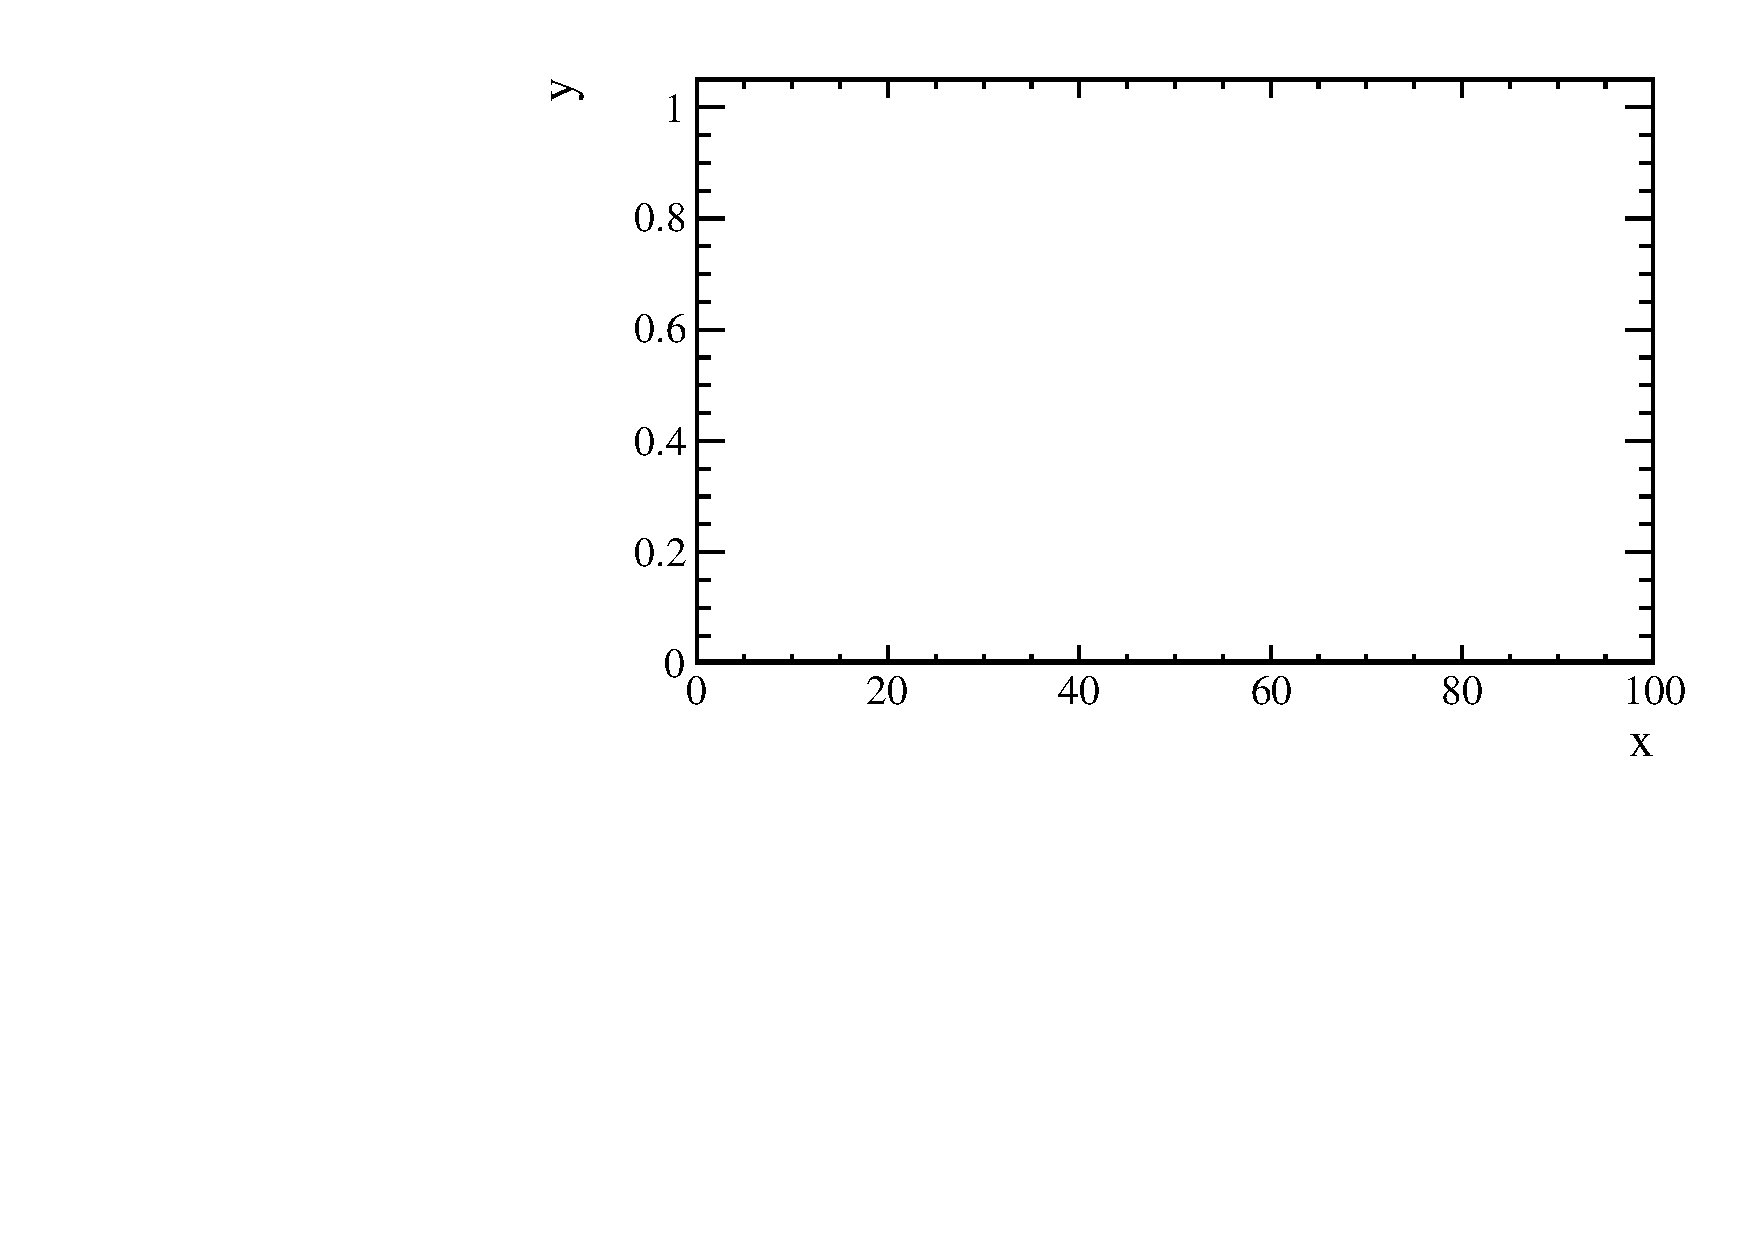
\includegraphics[width=0.48\textwidth]{blank}
    %\caption{
      %Evolution of the total efficiency for a \db with $\lifetime{\db}=100\ps$, where
      %black points indicate the sampled masses, and the red line is the interpolated cubic spline
      %intersecting each point.
    %}
    %\label{fig:eff:spline}
  %\end{center}
%\end{figure}

%\subsection{Normalization channel}
%The normalization channel is restricted in \qsq region, between 1.1 and $6.0\gevgev$.
%Using generator level simulation, it is determined that $(20.11\pm0.06)\%$ of generated events lie
%in this region.

\subsection[Mass resolution of the \db candidate]
{Mass resolution of the $\boldsymbol{\db}$ candidate}
The size of the signal and background regions are defined in terms of the local mass resolution,
which varies across the whole mass range.
To understand the evolution of \sigmam, the mass distribution of various signal samples are fitted
to a function constructed as the sum of two Gaussian distributions with the same mean.
Fitted distributions are used to define the $2\sigma$ intervals, and then each point is
intersected with a cubic spline.
Figure~{fig:param:mass} shows the resulting spline.
The mass resolution is observed to be
\approx$1\mev$ for very low \mass{\db} and quickly increases to a plateau around $2\sigma=15\mev$
before dropping off again because the invariant mass of the $\kpi\mumu$ system is constrained to
the known \Bd mass.

\begin{figure}
  \begin{center}
    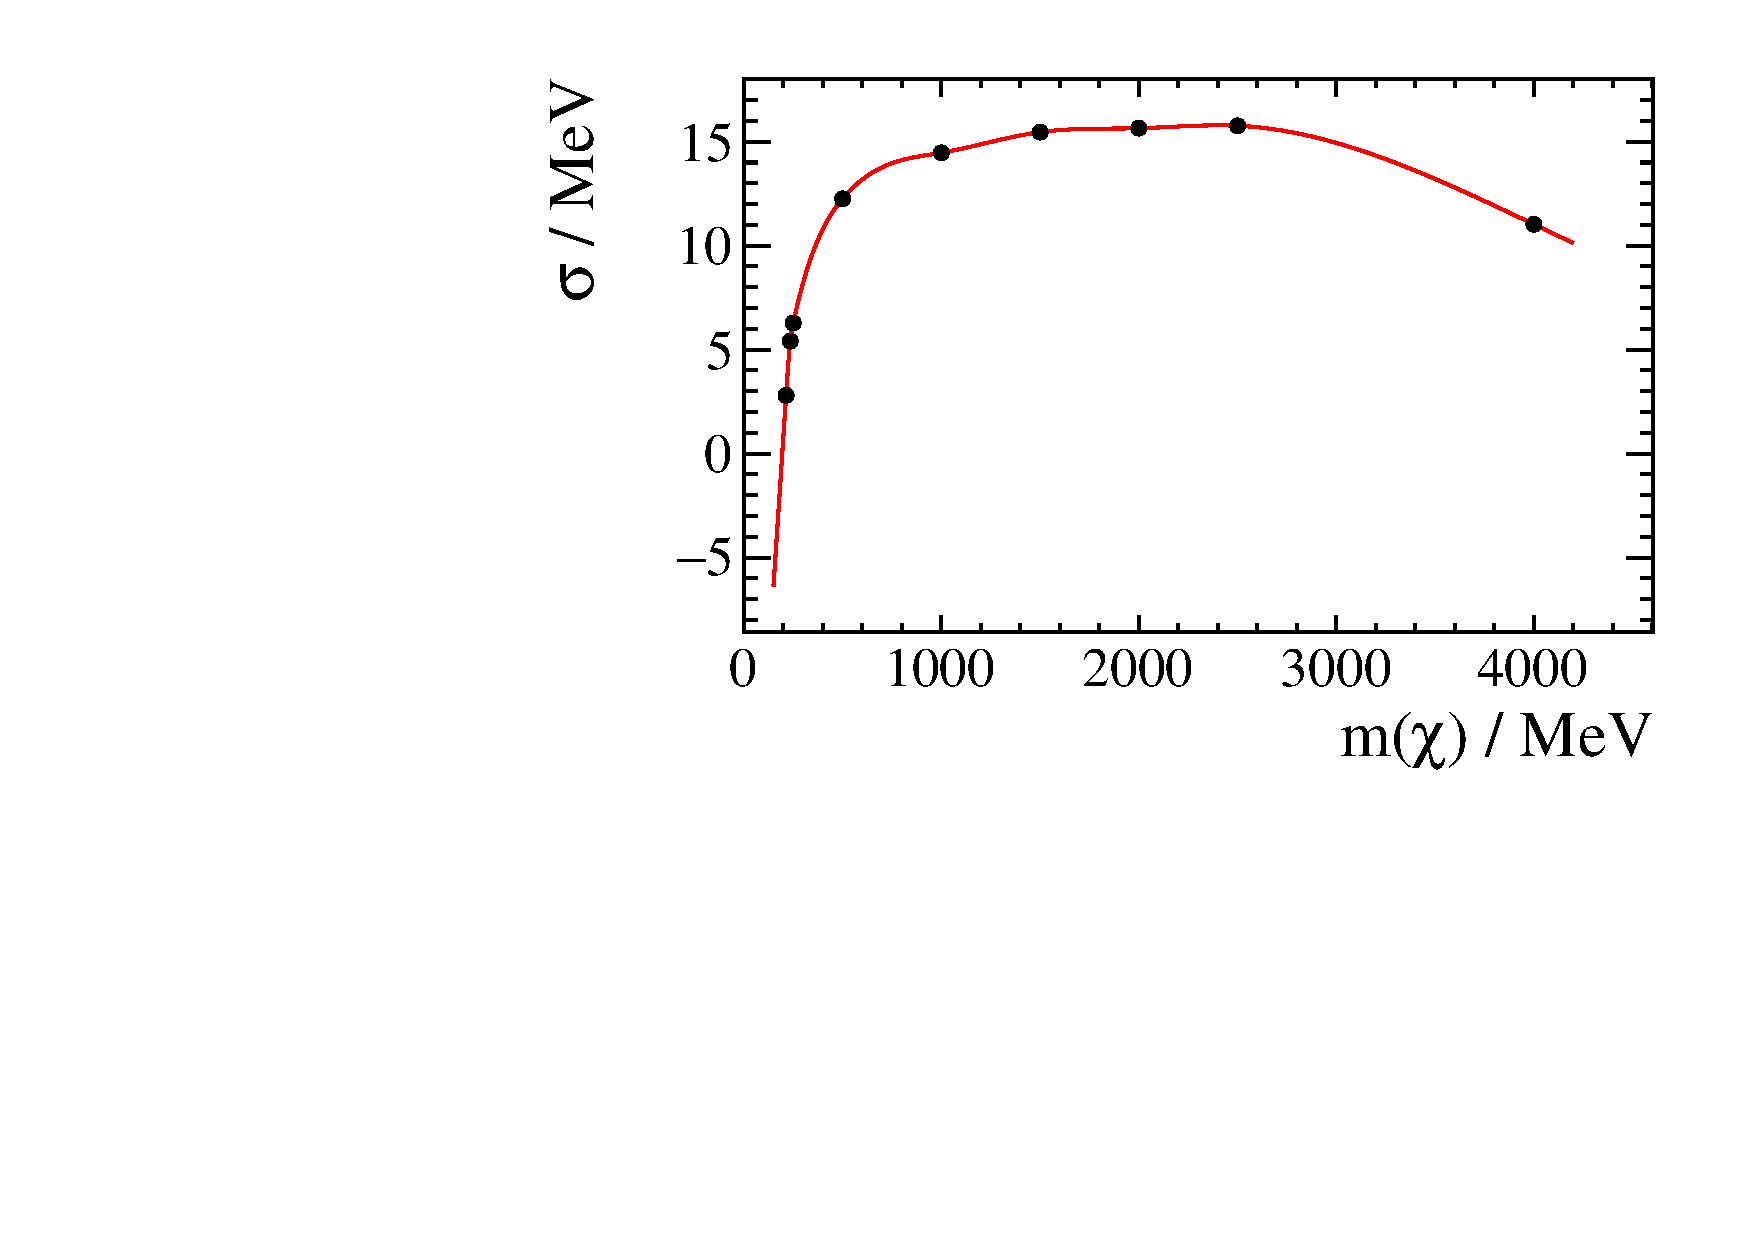
\includegraphics[width=0.48\textwidth]{spline_mass_sig}
    \caption[Evolution of mass resolution with \mass{\db}]
    {
      Evolution of $2\sigmam$ as a function of mass.
      The mass distribution of each simulated signal sample is fit to a distribution constructed of
      two Gaussian functions with the same mean, the value of $2\sigmam$ is then extracted by
      finding the $2\sigma$ interval of the fitted distribution.
      Each black point shows the value of $2\sigmam$ for a given simulated \btokstrdb sample, and
      the red line is the cubic spline intersecting each point.
    }
    \label{fig:param:mass}
  \end{center}
\end{figure}

%The local dimuon mass resolution varies as a function of $\mass{\mumu}$, and since the size of the
%signal and background regions are defined in terms of the
%The resolution for each simulated sample is found by fitting the mass spectrum to a
%double Gaussian function.
%The width of a distribution defines the resolution for a given mass, and spline interpolation is
%again used to obtain the resolution for all $m_\mumu$.
%Figure~\ref{fig:massres} shows the individual fits, while \Fig{fig:eff:spline:mass} shows
%the mass resolution as a function of mass.

%\begin{figure}
  %\begin{center}
    %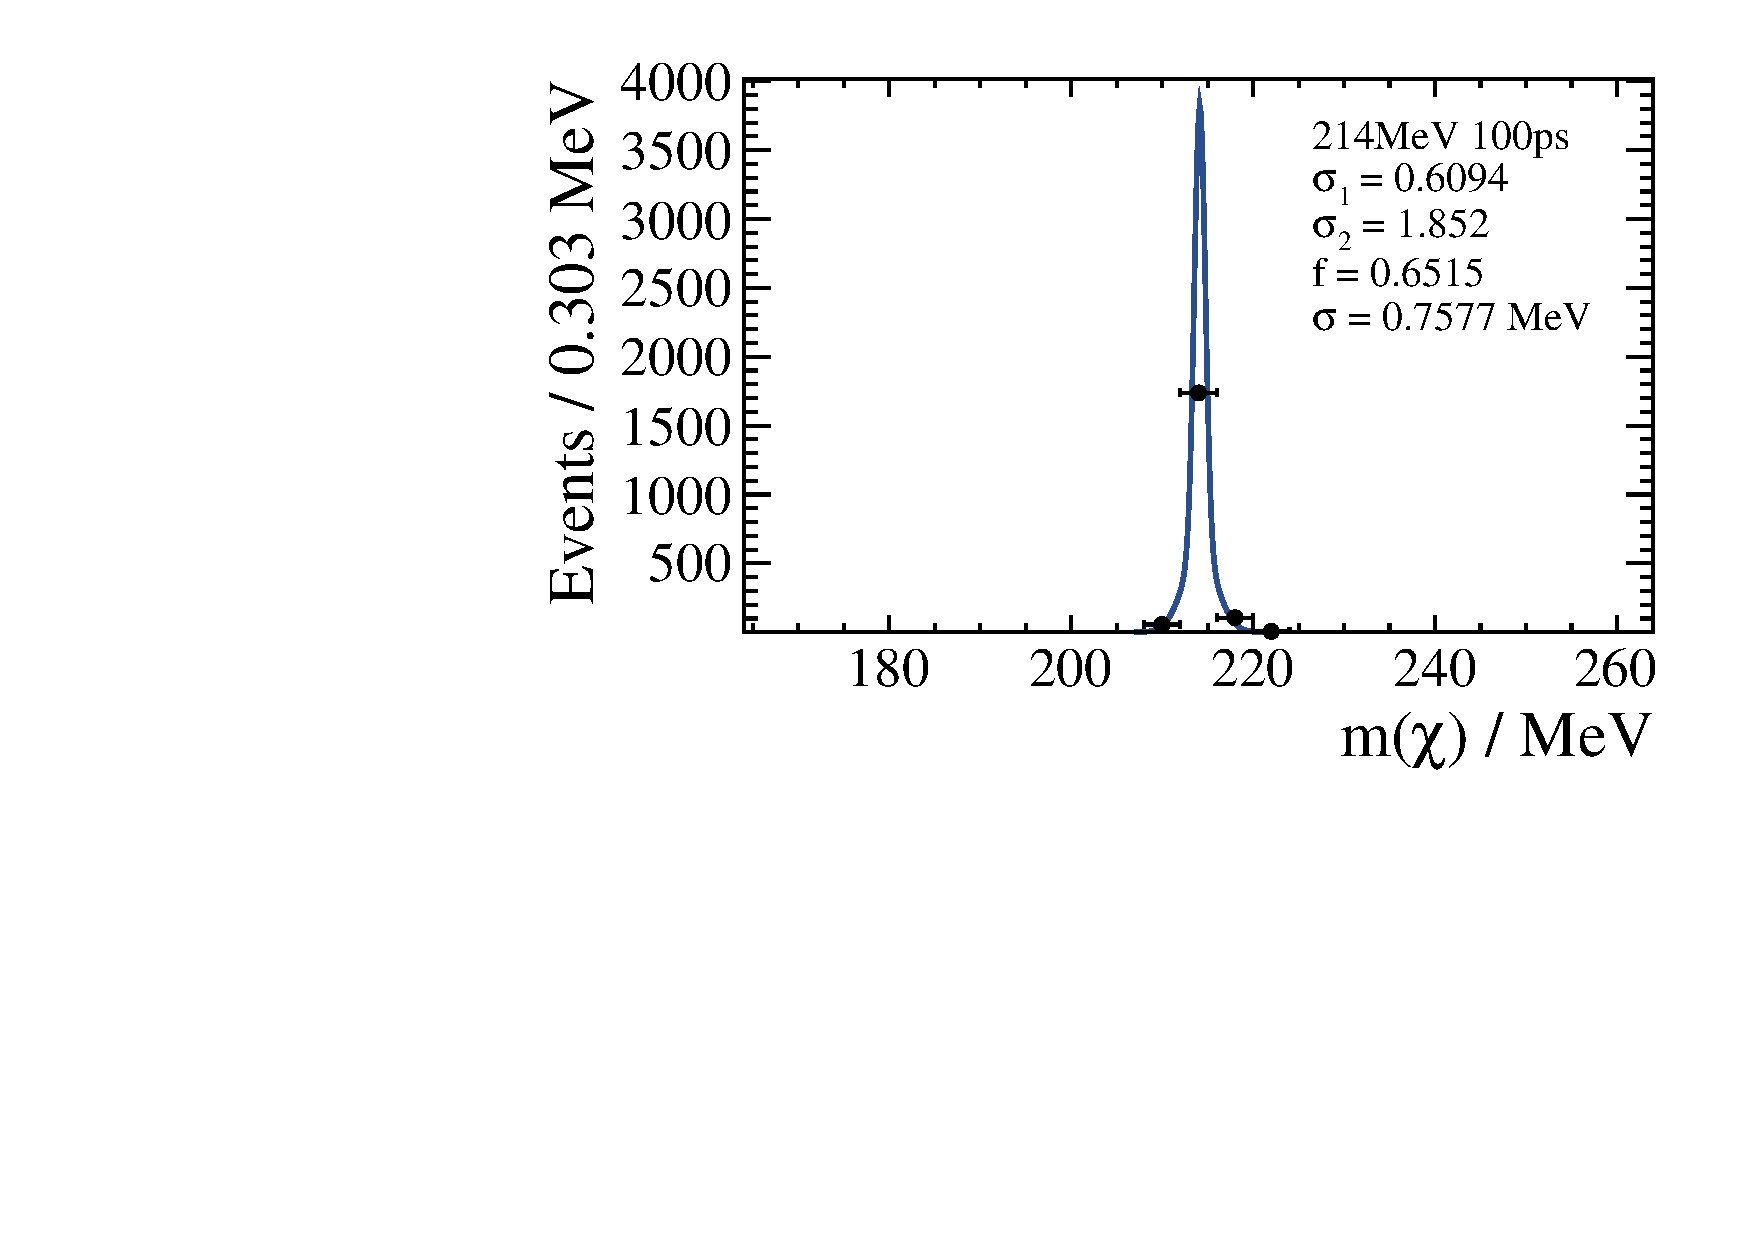
\includegraphics[width=0.42\textwidth]{anaResMass_214_100}
    %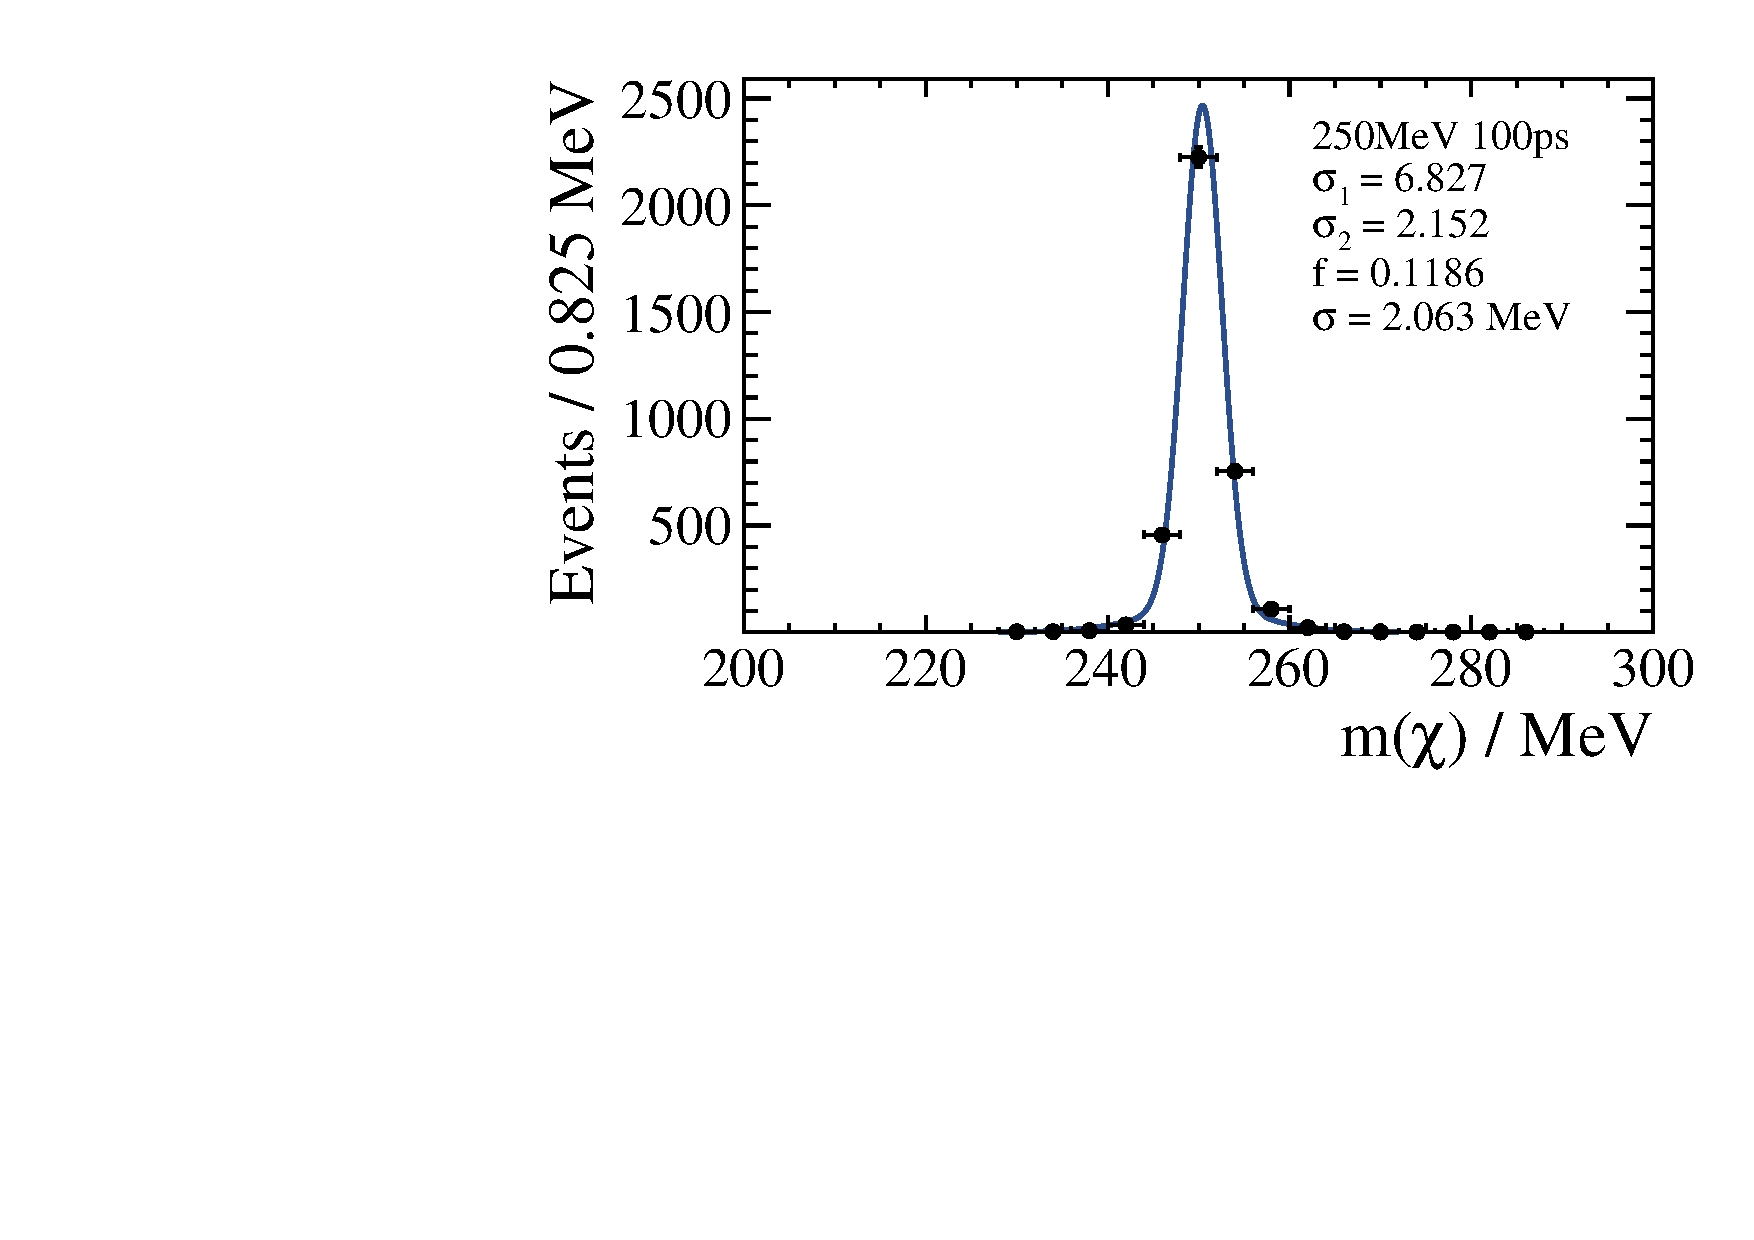
\includegraphics[width=0.42\textwidth]{anaResMass_250_100}
    %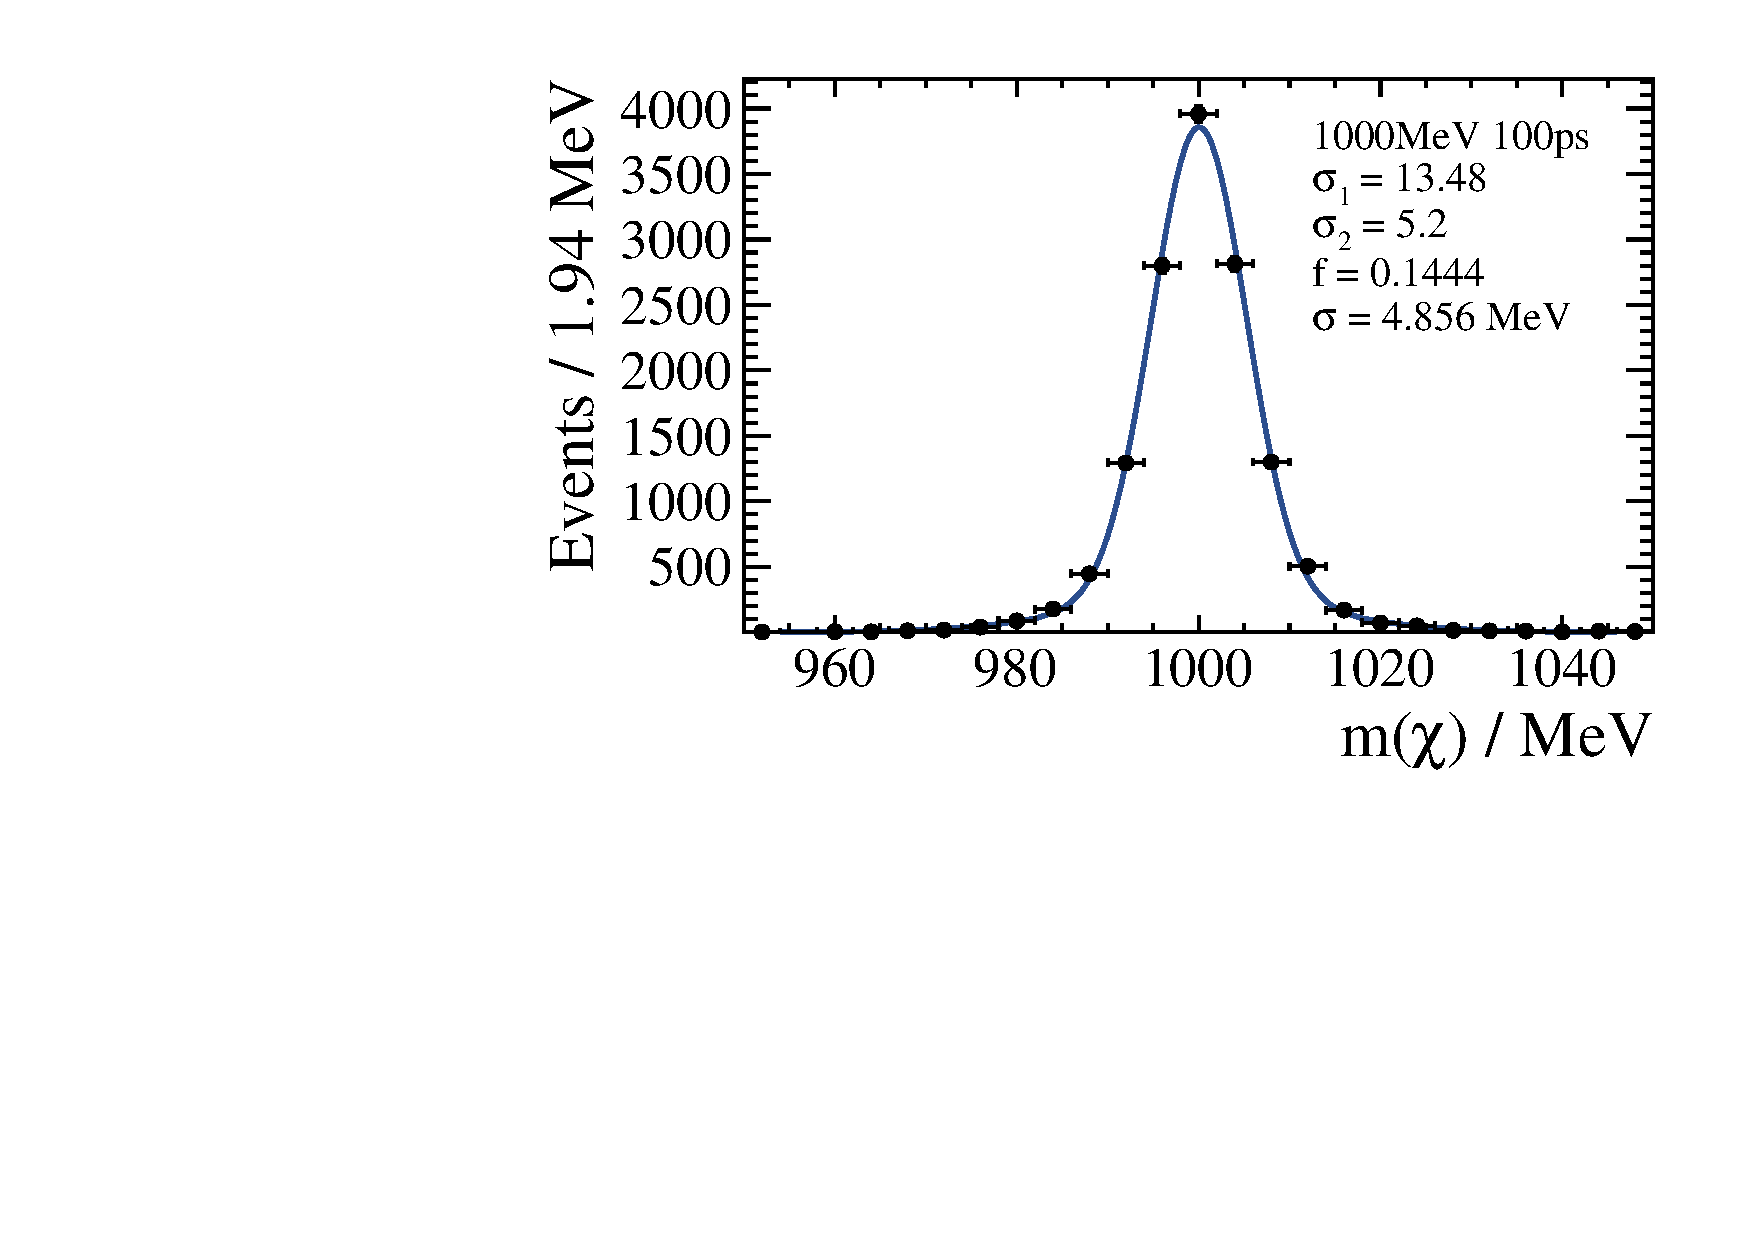
\includegraphics[width=0.42\textwidth]{anaResMass_1000_100}
    %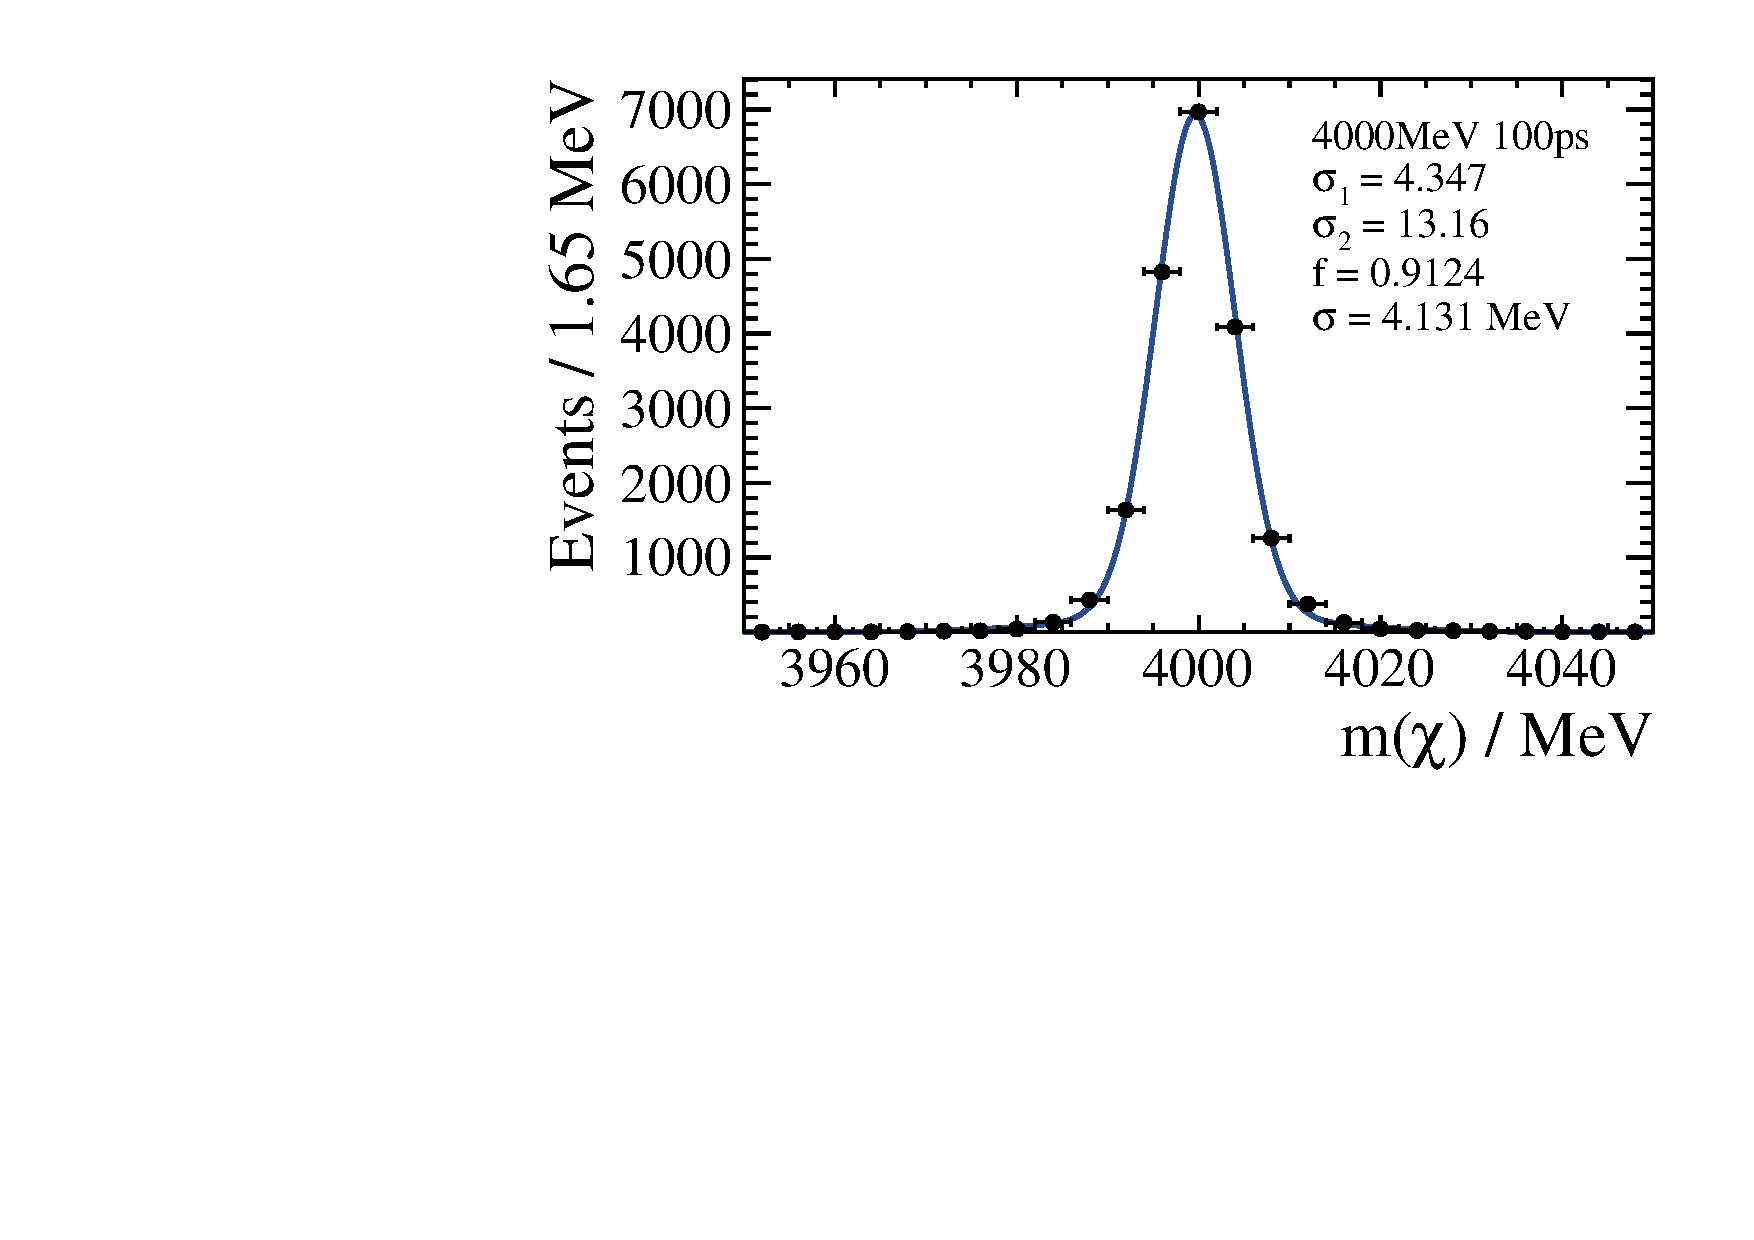
\includegraphics[width=0.42\textwidth]{anaResMass_4000_100}
  %\end{center}
  %\caption{
    %Mass resolution for different values of \mdb, each dataset is fit to a double Gaussian
    %function.
  %}
  %\label{fig:massres}
%\end{figure}


\subsection[Lifetime resolution of the \db candidate]
{Lifetime resolution of the $\boldsymbol{\db}$ candidate}
Similar to finding the mass resolution as a function of mass, the evolution of the lifetime
distribution is obtained by extracting the $3\sigmat$ limits from fitted distributions at known \db
mass points.
Splines are then used to interpolate to all values of \mass{\db}.
For each \btokstrdb sample with $m\leq250\mev$,
$\Delta\tau=\tau^\mathrm{meas}_{\db}-\tau^\mathrm{true}_{\db}$ distribution is fit to the sum of
two Gaussian functions with the same mean.
In samples with $\mass{\db}<250\mev$ the $\Delta\tau$ distribution is observed to be significantly
distorted from a simple double Gaussian.

When a \db is produced near the dimuon mass threshold when the \db decays into two muons, the
daughter particles are produced at rest in the frame of the \db.
Therefore, the two muons have a very narrow opening angle, $\theta_\mathrm{open}$ in the lab frame
and the separation of their hits in the \velo are
comparable to the resolution of the \velo strips and leads to poor spatial resolution of
the \db decay vertex position.
The resolved muon hits in the \velo are pushed further downstream, such that
$\tau^\mathrm{meas}_{\db}>\tau^\mathrm{true}_{\db}$.

The effect of a small opening angle can be seen by comparing the measured and true opening angle
distributions for simulated decays of \btokstrdb, where $\mass{\db}=214\mev$.
Figure~\ref{fig:opening:gen} shows that
for $\theta_\mathrm{open}\lesssim0.002\rad$ a significant discrepancy between the distributions of
$\thetaopen^\mathrm{true}$ and $\thetaopen^\mathrm{measured}$.
In the same figure, the evolution of \thetaopen with \mass{\db} at generator level is shown, it can
be seen that when $\mass{\db}=250\mev$, the opening angle is predominantly larger than $0.002\rad$.
%Applying a cut to \thetaopen is very signal inefficient, so instead
%it can be seen that there is no bias once the \mumu opening angle exceeds $\sim0.002$ radians.
%Vetoing all events below this threshold is a very inefficient solution at low dimuon
%masses, (see Fig.~\ref{fig:opening:gen}).
%Instead, the bias is accounted for, as described below.

%The lifetime resolution is obtained by fitting
%\Fig{fig:taures:zoom}, and finding the $3\sigma$ limits of these
%probability density functions.
%For $m_{\mumu} > 250\mev$ the $\tau$ measurement is unbiased and has nearly uniform resolution.
%However, for dimuon masses close to threshold, where the break up momentum is small, the lifetime
%measurement is biased and less precise.
%There is a strong difference between the resolution in the  214 and the $250\mev$ samples.
%For this reason, small samples of simulated signal events were produced at 220 and 235\mev to aid
%with the understanding of the detector response in this dimuon mass region.

\begin{figure}
  \begin{center}
    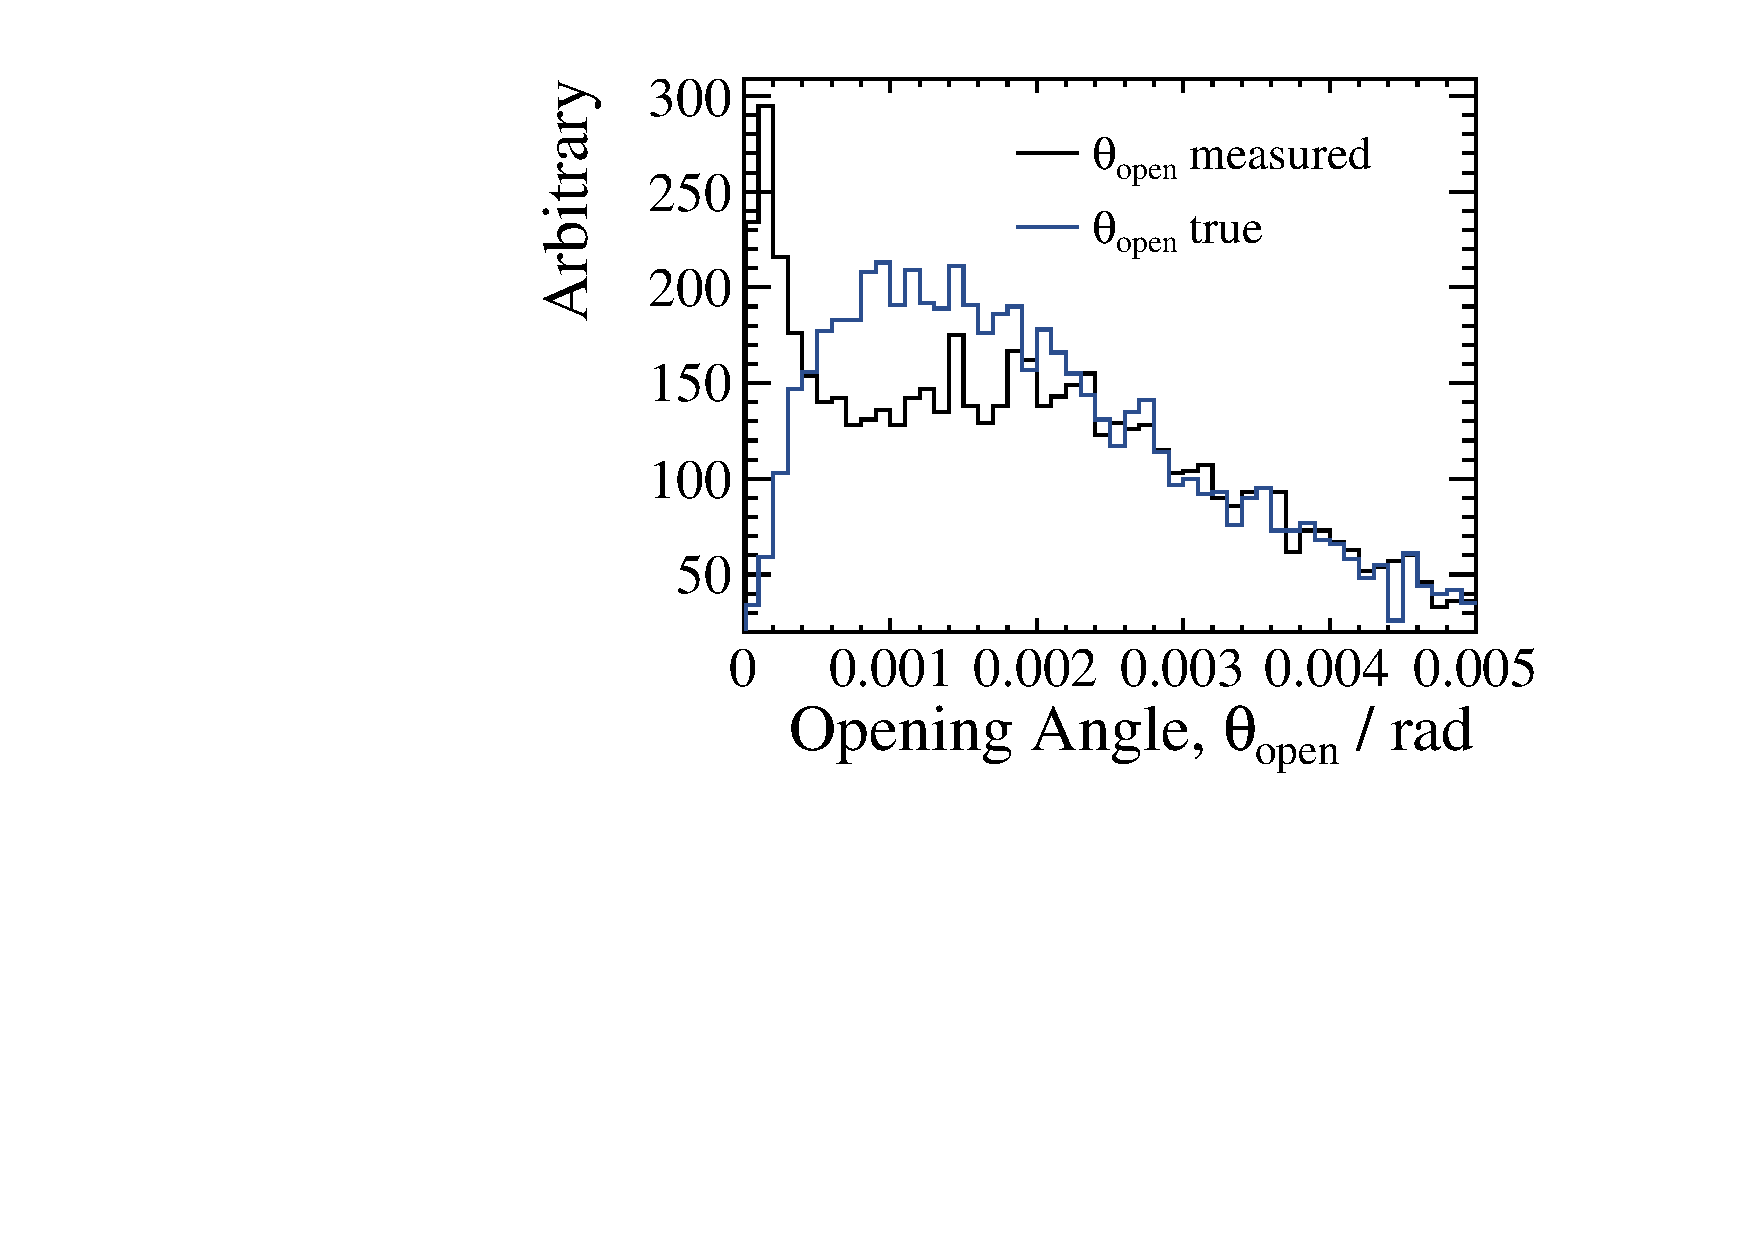
\includegraphics[width=0.48\textwidth]{ana214Opening}
    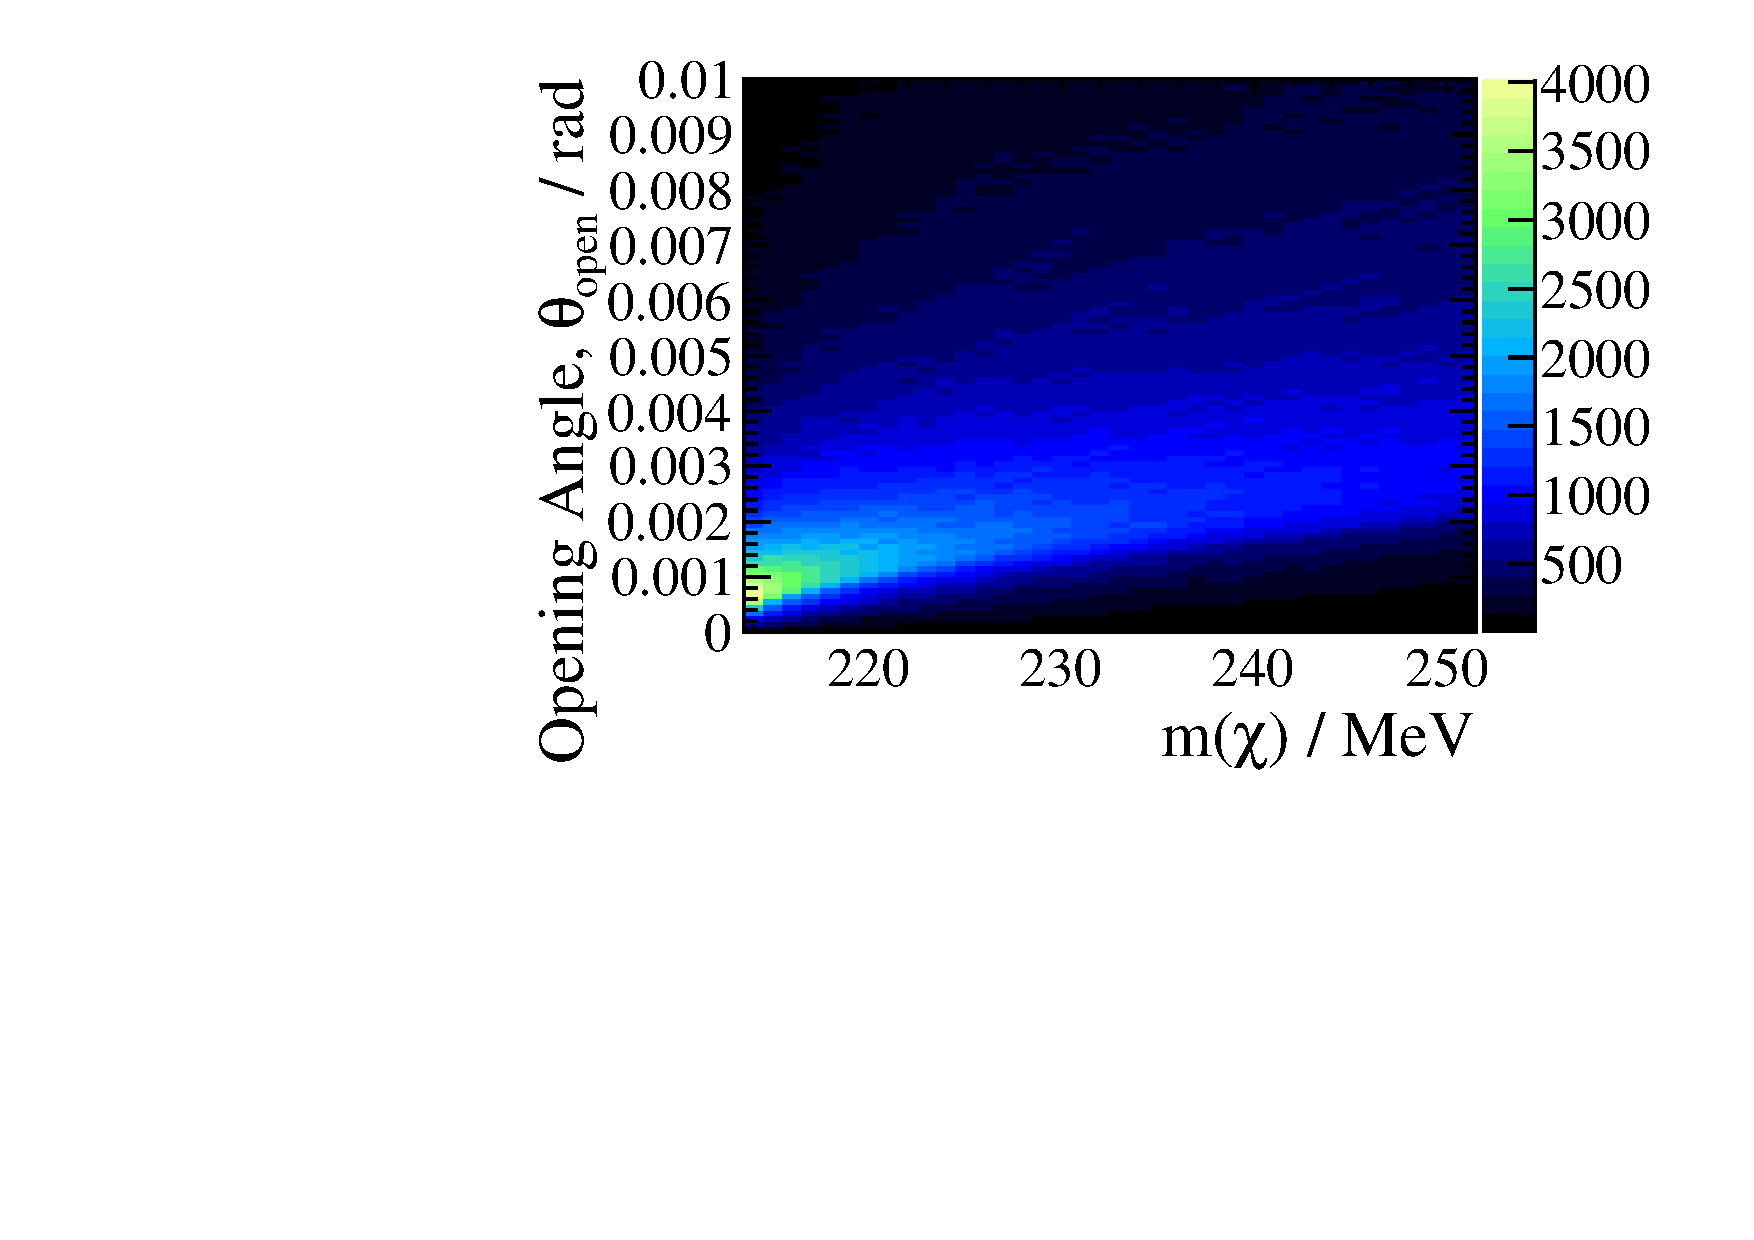
\includegraphics[width=0.48\textwidth]{anaGenLevelOpening}\\
  \end{center}
  \caption{\small
    The opening angle of the two muons decaying from the \db is highly dependent on \mdb; for low
    dimuon masses the opening angle measurement is biased.
    For $\mdb=214\mev$ the difference between generated and reconstructed opening angles are shown,
    (left) the greatest difference being below $\theta_\mathrm{open}=0.002$.
    Generator level distributions of opening angles for a range of masses,
    (right) show that most \db decays have $\theta_\mathrm{open}>0.002$ for
    $\mdb\gtrsim235\mev$.
  }
  \label{fig:opening:gen}
\end{figure}

The discrepancy between real and true opening angle can be verified using data
from a decay channel with very high statistics, such as the opening angle of the \kpi system in
the decay \decay{\Bd}{\kpi\mumu} for for $m_{\kpi}<\mev$.
Figure~\ref{fig:oa:2d} shows that the opening angle of the \kpi system
is very low, and a similar peak at $\thetaopen=0$ when $m_{\kpi}$ is near threshold,
($m_{\Kp} + m_{\pim} = 633.3\mev$).
A one dimensional plot of the opening angle for $m_{\kpi}<640\mev$ is shown in \Fig{fig:db:openkpi}.

\begin{figure}
  \begin{center}
    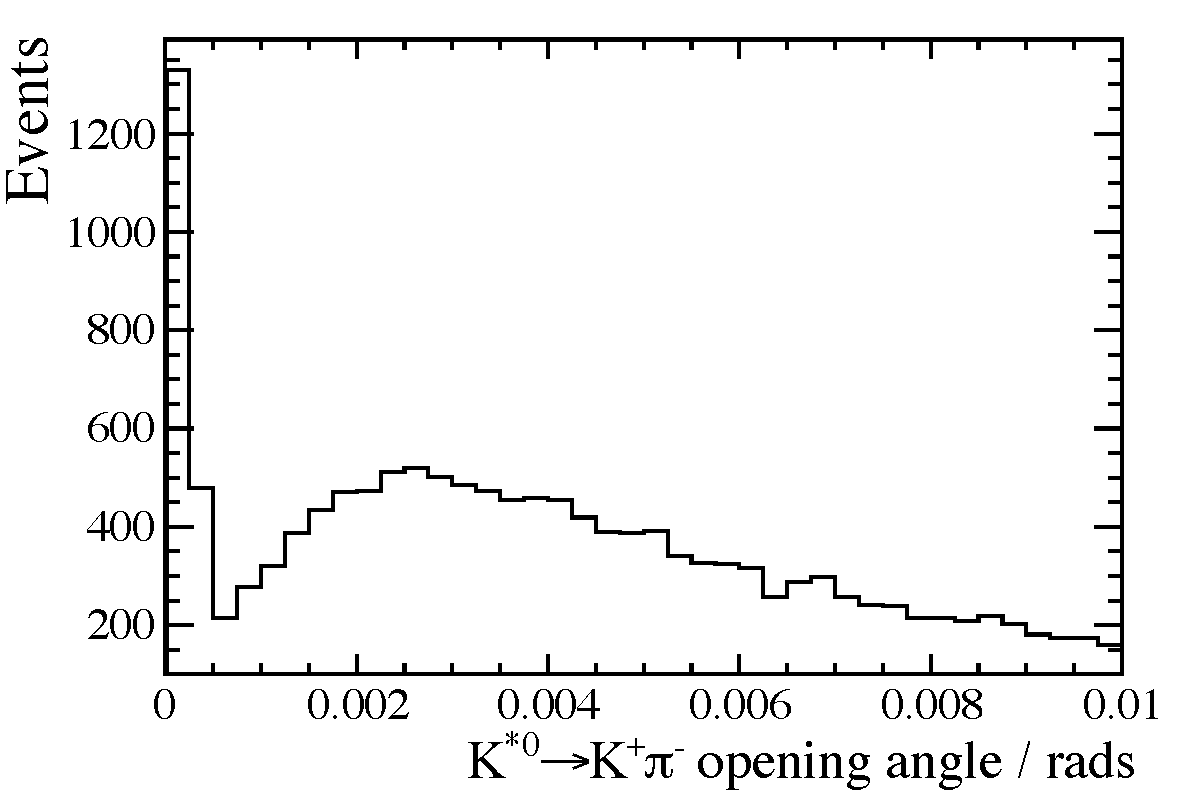
\includegraphics[width=0.48\textwidth]{opening_angle_data}
    %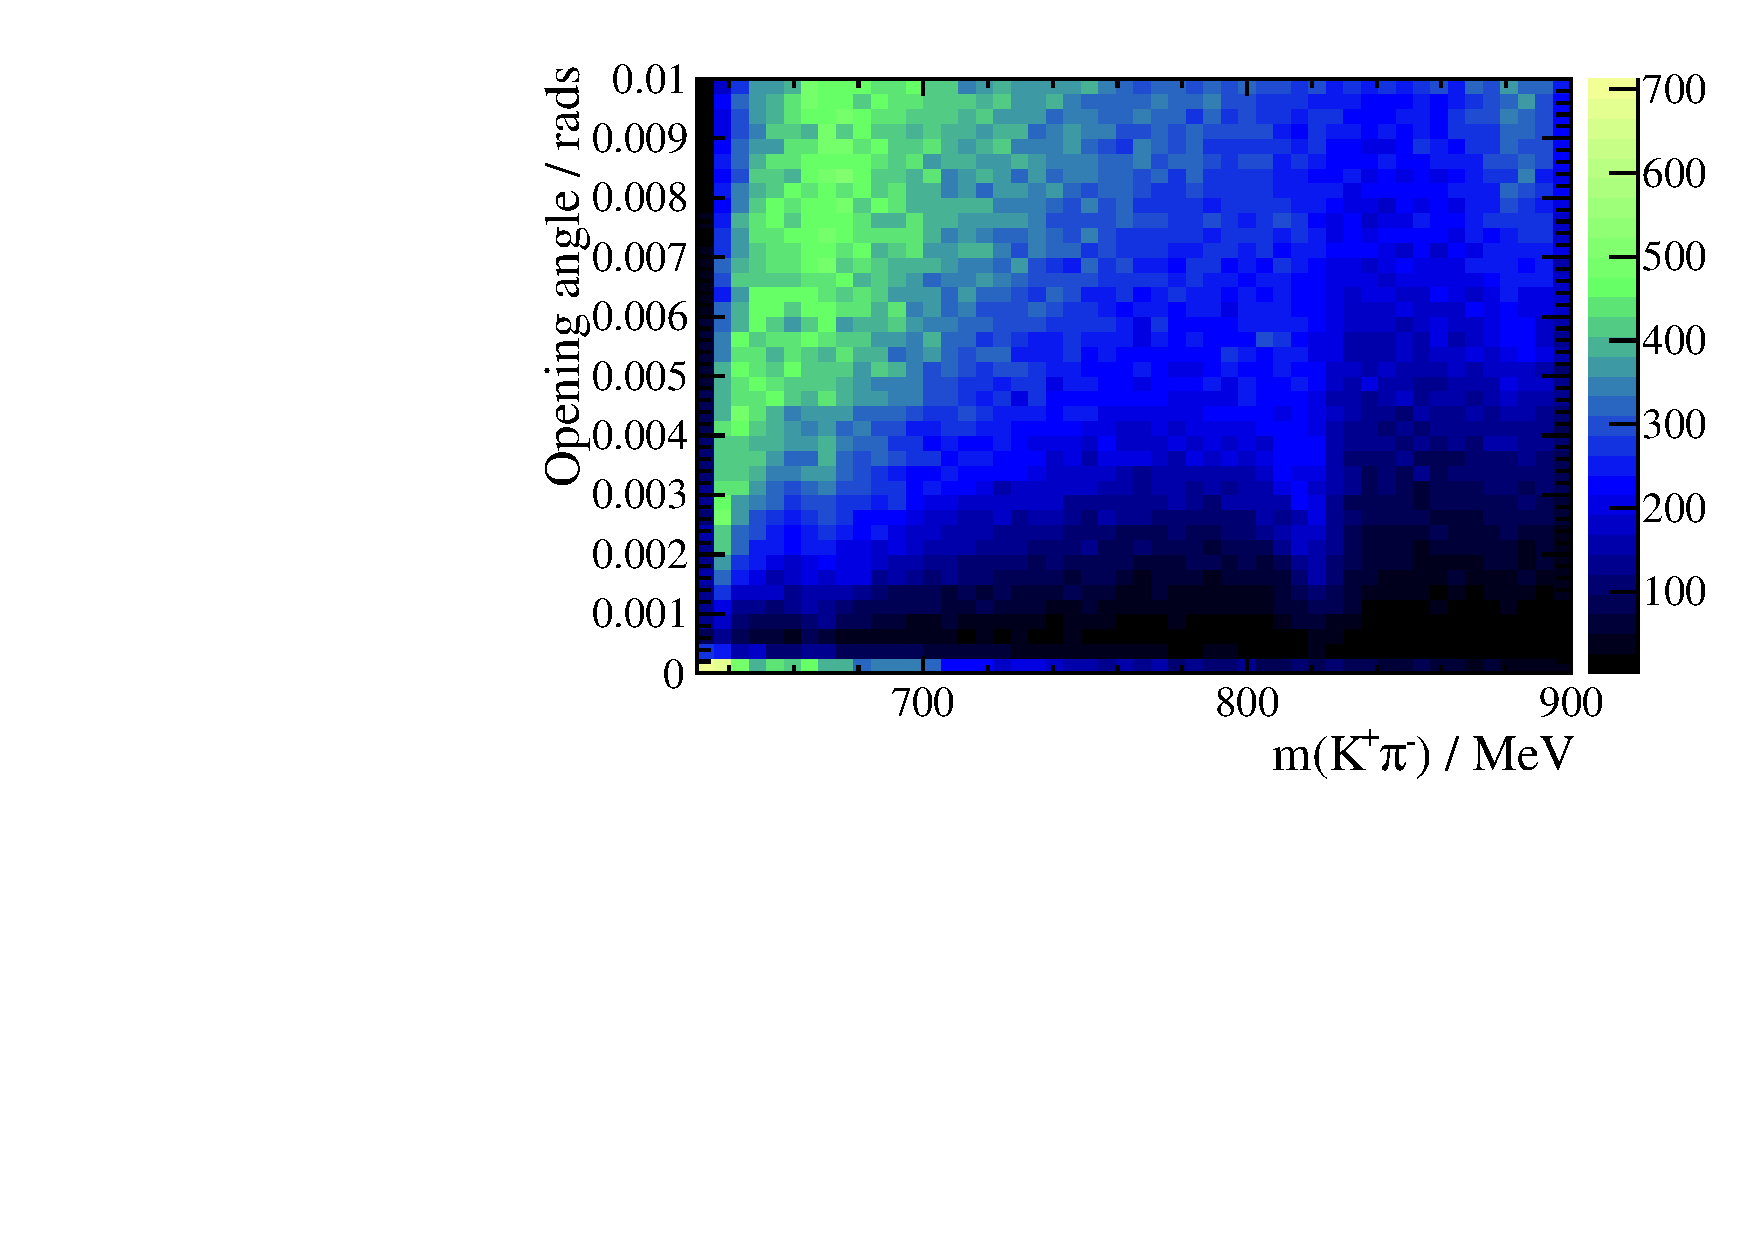
\includegraphics[width=0.48\textwidth]{opening_angle_data_2d}
    \caption[Opening angle of \kpi]
    {
      Opening angle of the \kpi system in \decay{\Bd}{\kpi\mumu}, where the invariant mass of the
      \kpi system is close to threshold.
    }
    \label{fig:db:openkpi}
  \end{center}
\end{figure}

Applying a cut to remove events where \thetaopen is small would be very inefficient for a low mass
\db, and therefore the function used to fit $\Delta\tau$ is modified to account for the positive
skew.
For simulated samples generated with $\mass{\db}<250\mev$ the wider of the two Gaussian functions
is modified to incorporate an exponential tail
extending to high $\Delta\tau$ and allowing the mean of both Gaussians by allowing the mean to
shift from zero.
Fits to $\Delta\tau$ from \btokstrdb samples with different values of \mass{\db} are shown in
\Fig{fig:taures:zoom}.
Accounting for this effect allows the $\pm3\sigma_\tau$ values to be taken directly from the fits.


\begin{figure}
  \begin{center}
    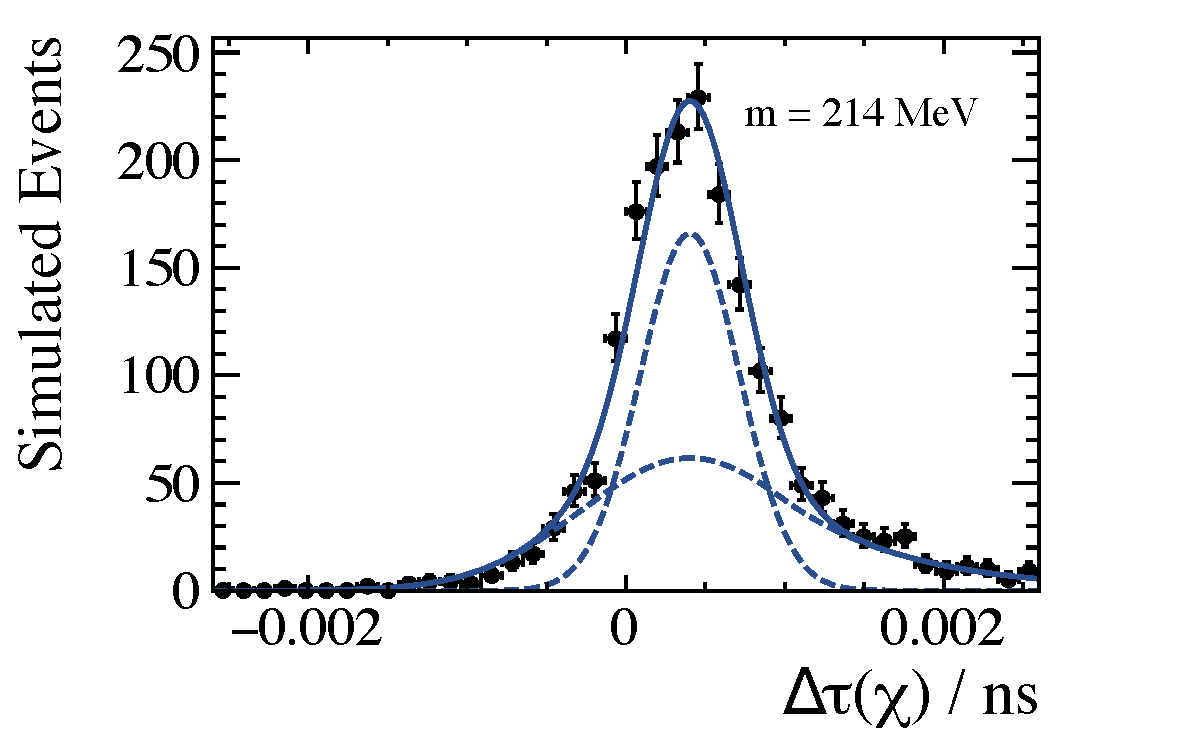
\includegraphics[width=0.42\textwidth]{anaTauResZoom_214}
    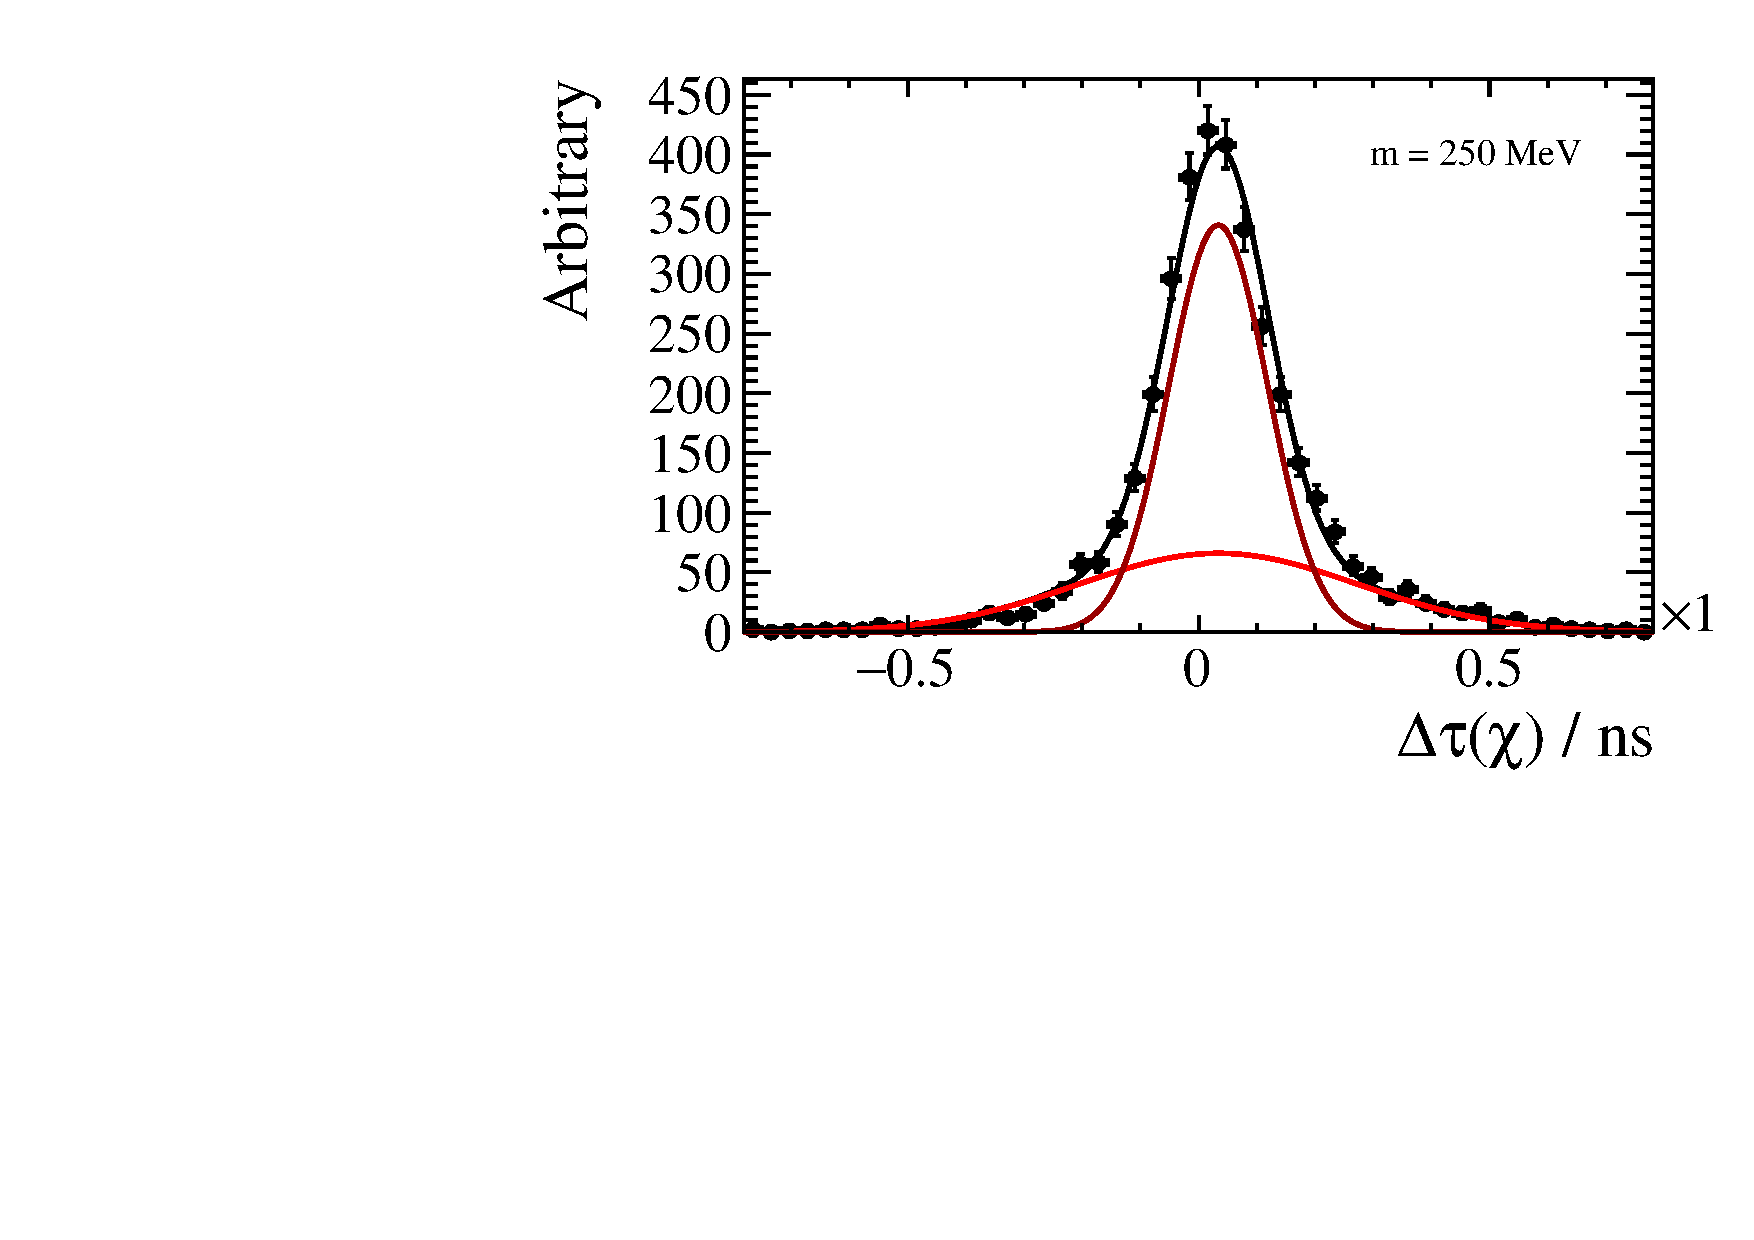
\includegraphics[width=0.42\textwidth]{anaTauResZoom_250}
    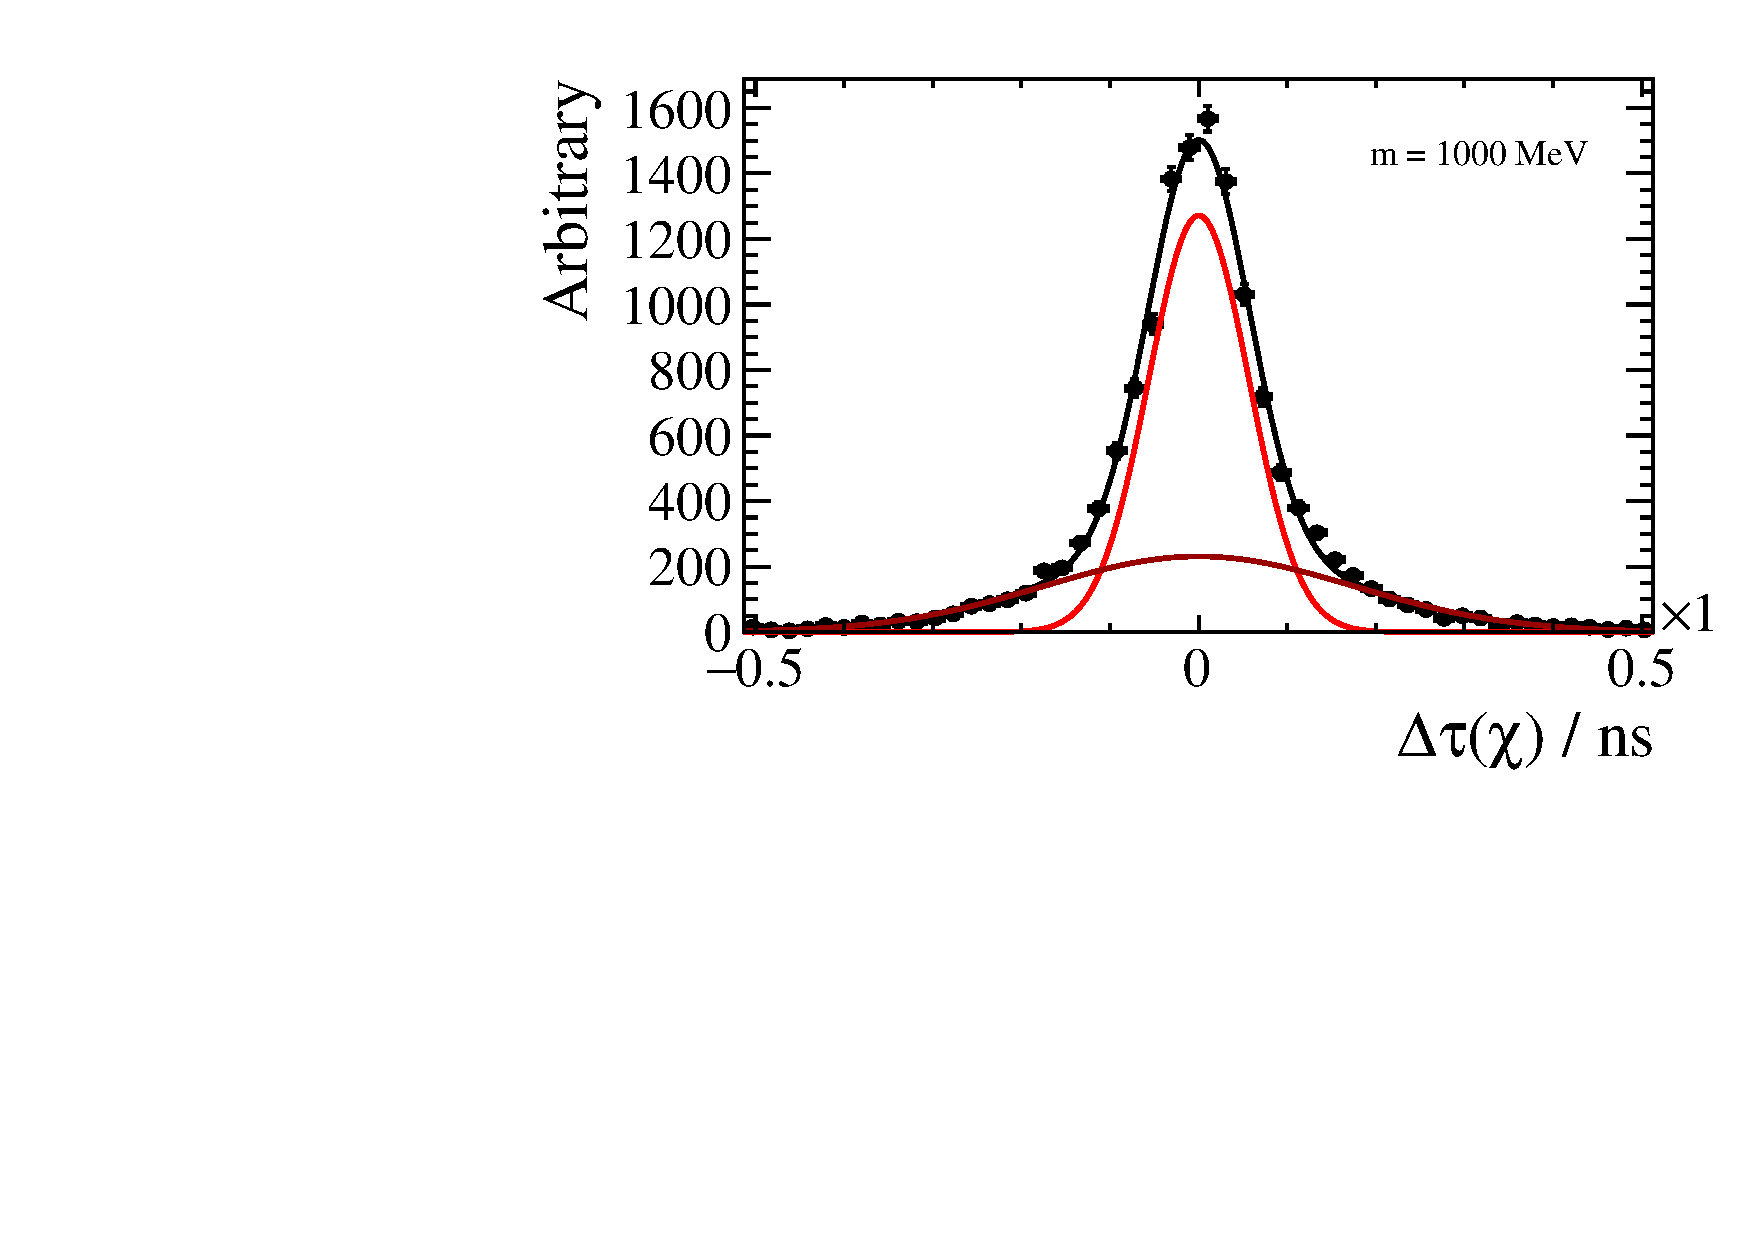
\includegraphics[width=0.42\textwidth]{anaTauResZoom_1000}
    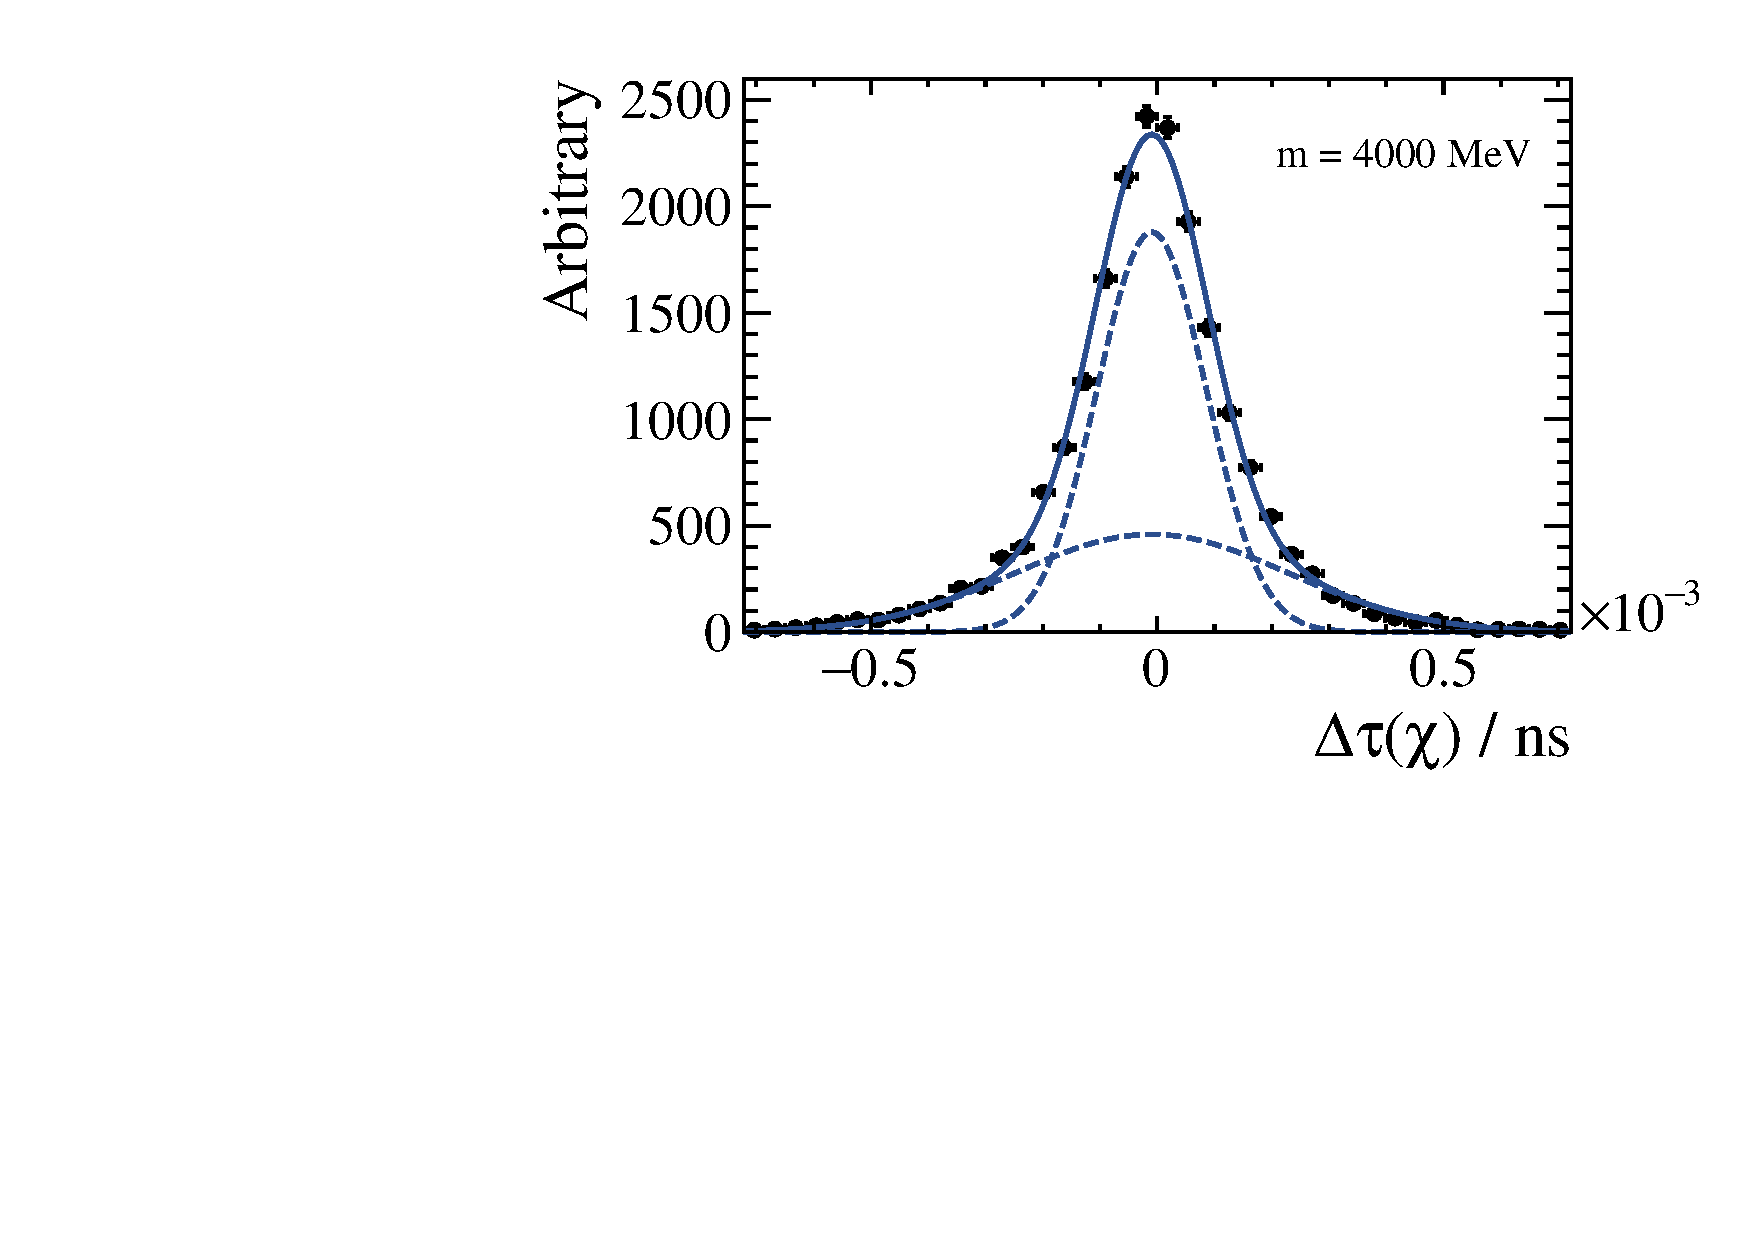
\includegraphics[width=0.42\textwidth]{anaTauResZoom_4000}
  \end{center}
  \caption[Fits to the lifetime resolution for simulated \db{s}]
  {
    Fits to the lifetime resolution parameter, $\Delta\tau$, for individual mass samples.
    Each fit for $m\geq250\mev$ is made using a double Gaussian function, and for $m<250\mev$ the
    wider Gaussian has an exponential tail on the right-hand side.
  }
  \label{fig:taures:zoom}
\end{figure}

The prompt region is defined by $-3\sigma_\tau<\tau_{\mumu}<3\sigma_\tau$ and the displaced region
by $\tau_{\mumu}>3\sigma_\tau$.
Figure~\ref{fig:eff:res} shows how $\sigma_\tau$ varies with mass, where each point comes from the
fits to $\Delta\tau$ described above, and linear spline interpolation is used to access
$\sigma_\tau$ at all values of \mass{t}.

%The lifetime resolution is calculated at each mass point using a fit to $\Delta\tau$.
%Each PDF is constructed as the sum of two Gaussian functions.
%However, for the reasons described above, the low mass ($<250\mev$) has a tail extending to high
%lifetimes, and therefore for these samples an exponential tail is added to the Gaussian with larger
%width.
%These fits are shown in \Fig{fig:taures:zoom}; the same distributions for flight distance (without
%fits) are shown in \Fig{fig:fd:zoom}.
%The $3\,\sigma$ lifetime resolution is calculated from the fitted PDFs, which are
%shown in Fig.~\ref{fig:eff:spline:res}.


\begin{figure}
  \begin{center}
    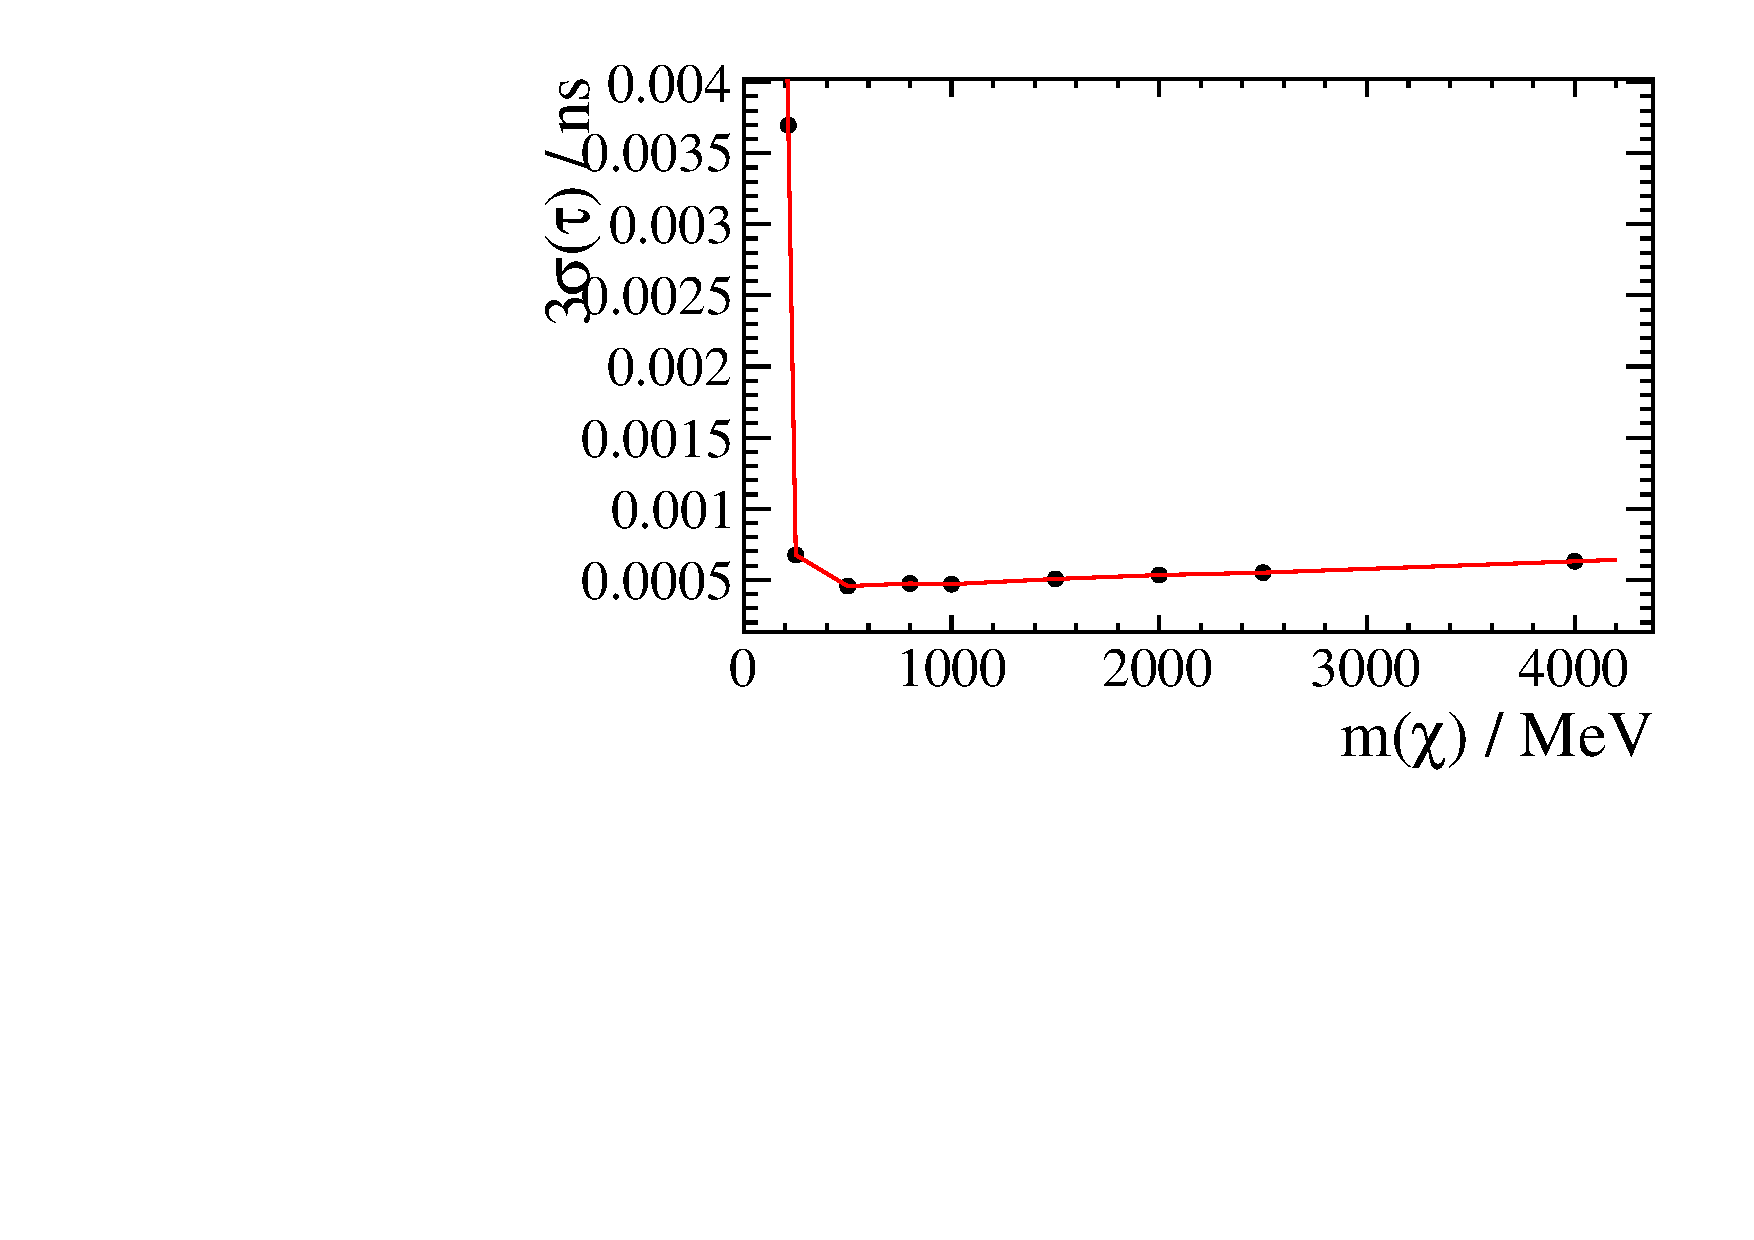
\includegraphics[width=0.48\textwidth]{spline_taures_upper}
    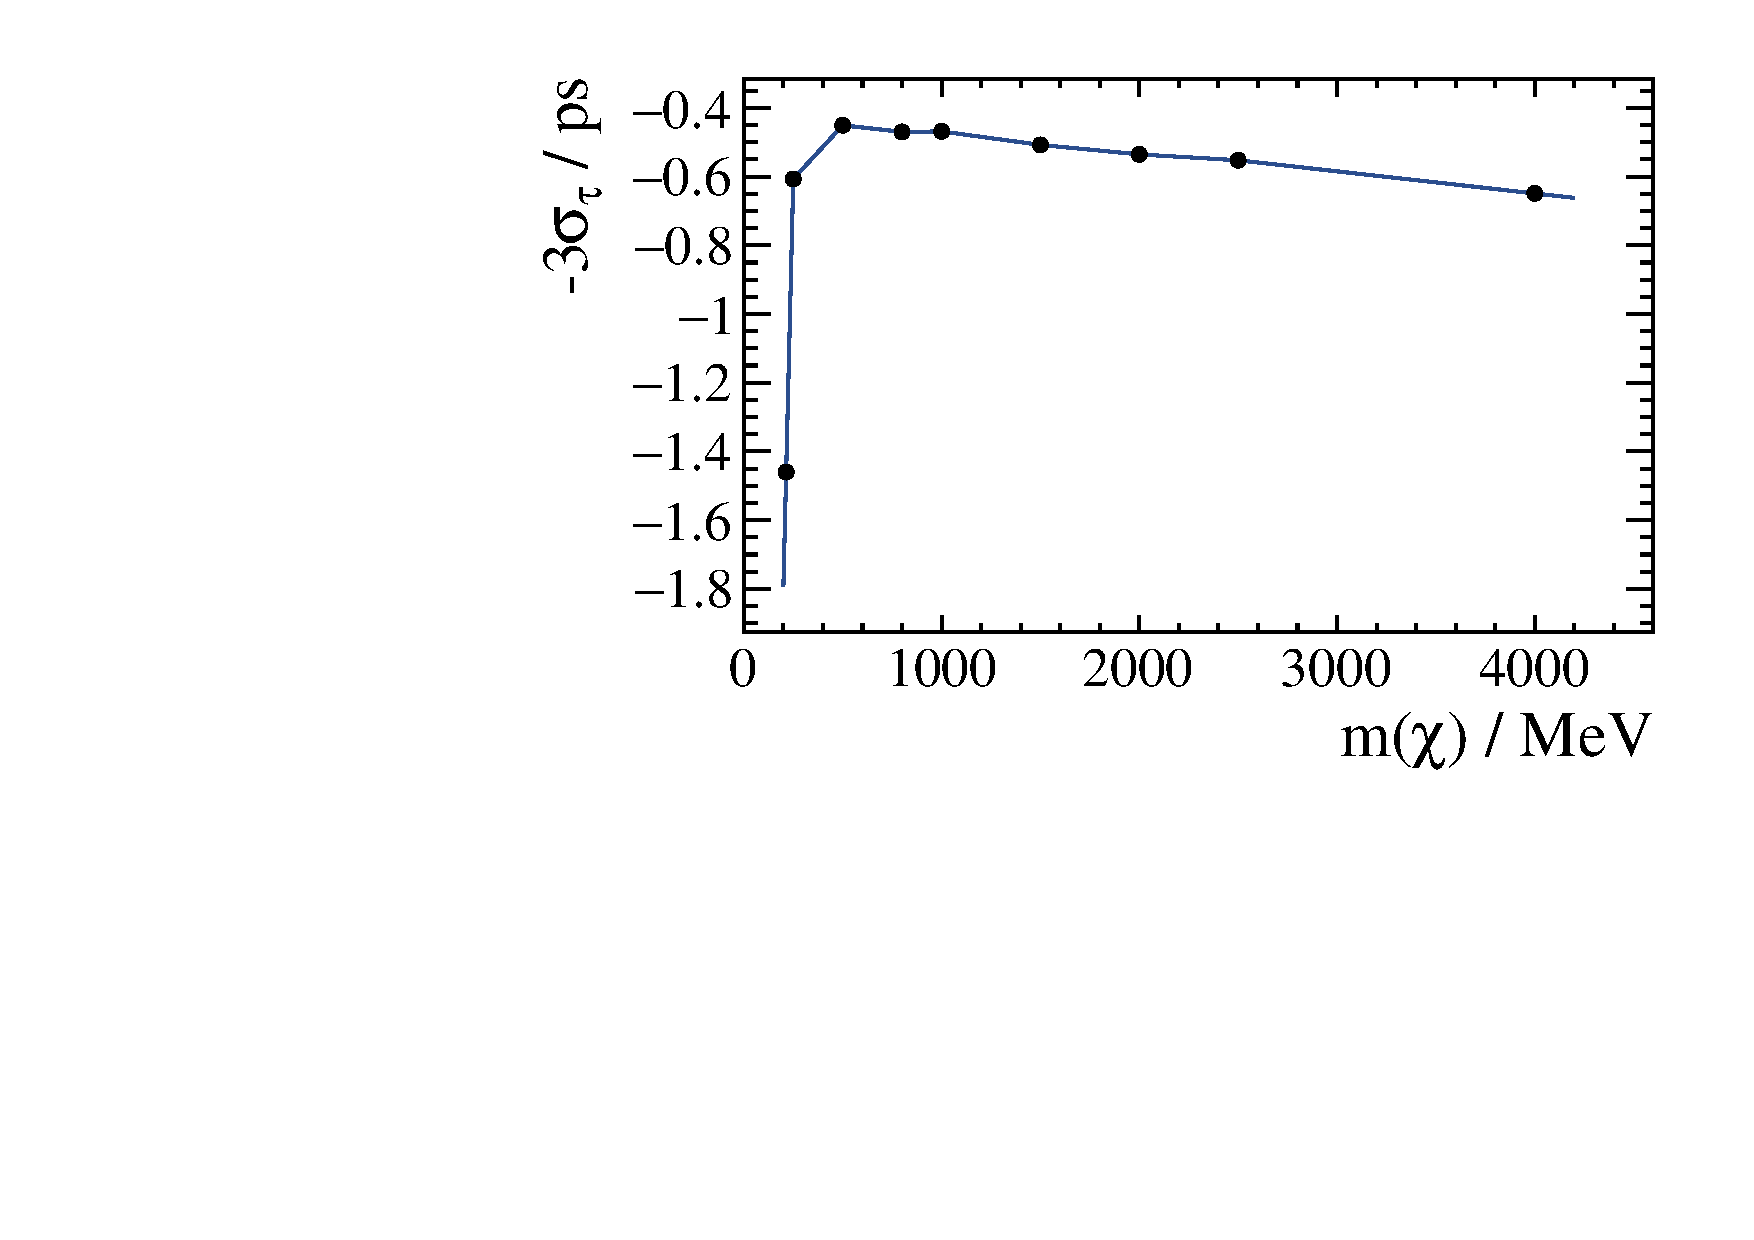
\includegraphics[width=0.48\textwidth]{spline_taures_lower}\\
    \caption[Parameterization of lifetime resolution as a function of \db mass]
    {
      Resolutions for the lifetime of a particle as a function of mass in the
      (upper left) positive and
      (upper right) negative directions at the $3\,\sigma$ levets, used to
      define prompt and displaced regions.
      (bottom) shows the $1\,\sigma$ mass resolution as a function of
      mass.
      The black points are from fitted values and the red lines show spline interpolation.
    }
    \label{fig:eff:res}
  \end{center}
\end{figure}



\subsection{Parameterizing the efficiency of the \db selection}
Setting limits for \db masses and lifetimes requires knowledge of the efficiency for any arbitrary
\db, as outlined in \Eq{eq:db:lim}.
To do this, the lifetime distribution for a given mass is fit to a simple function:
\begin{equation}
  \mathcal{T}(\tau) = f\mathcal{G}(\mu=0, \sigma) + (1-f)\exp\left(-\alpha\tau\right),
  \label{eq:eff:parameters}
\end{equation}
which depends upon only a few parameters: a $f$, $\sigma$, and $\alpha$.
There is excellent agreement between $\tau_\db$ distributions from simulated samples of \btokstrdb
and this simple parameterization, as shown in \Fig{fig:eff:fits}.

\begin{figure}
  \begin{center}
    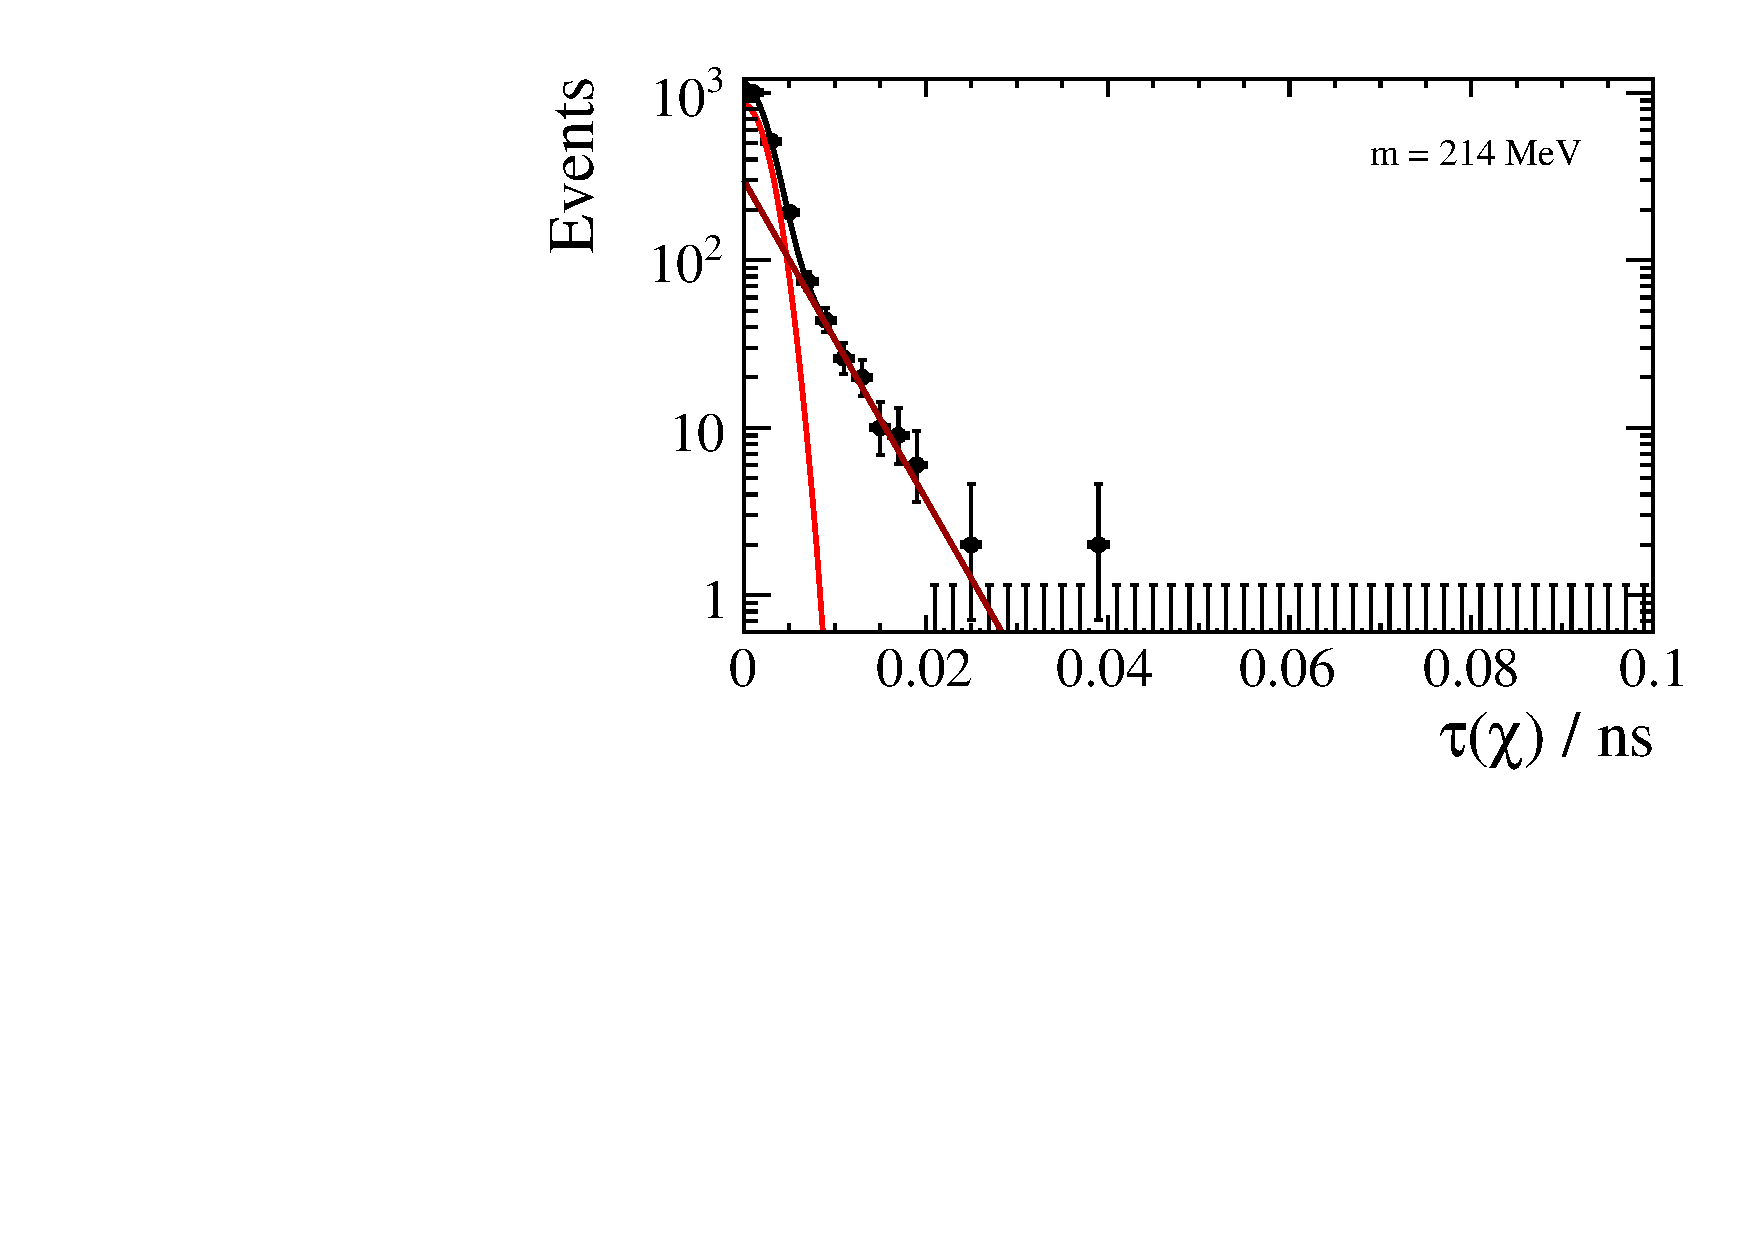
\includegraphics[width=0.48\textwidth]{anaTauEff_214}
    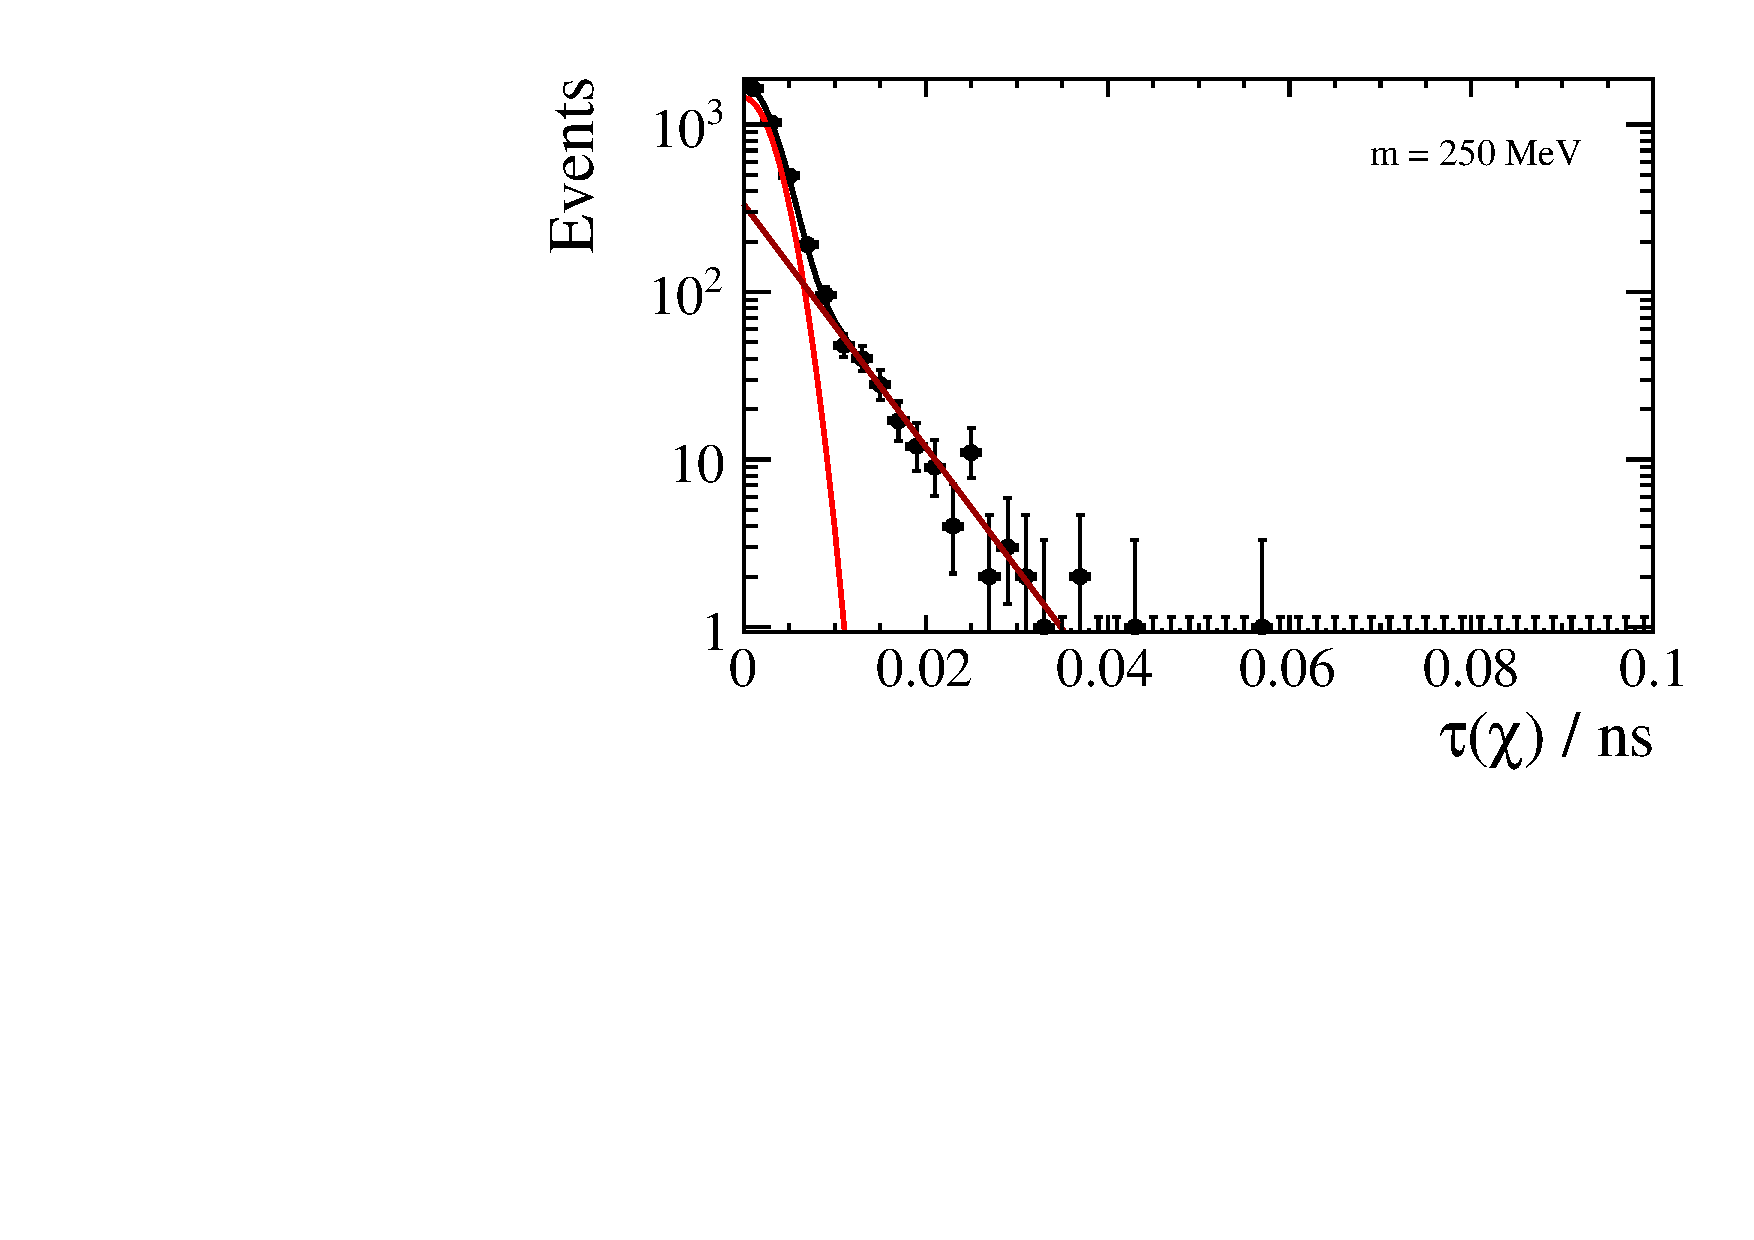
\includegraphics[width=0.48\textwidth]{anaTauEff_250}\\
    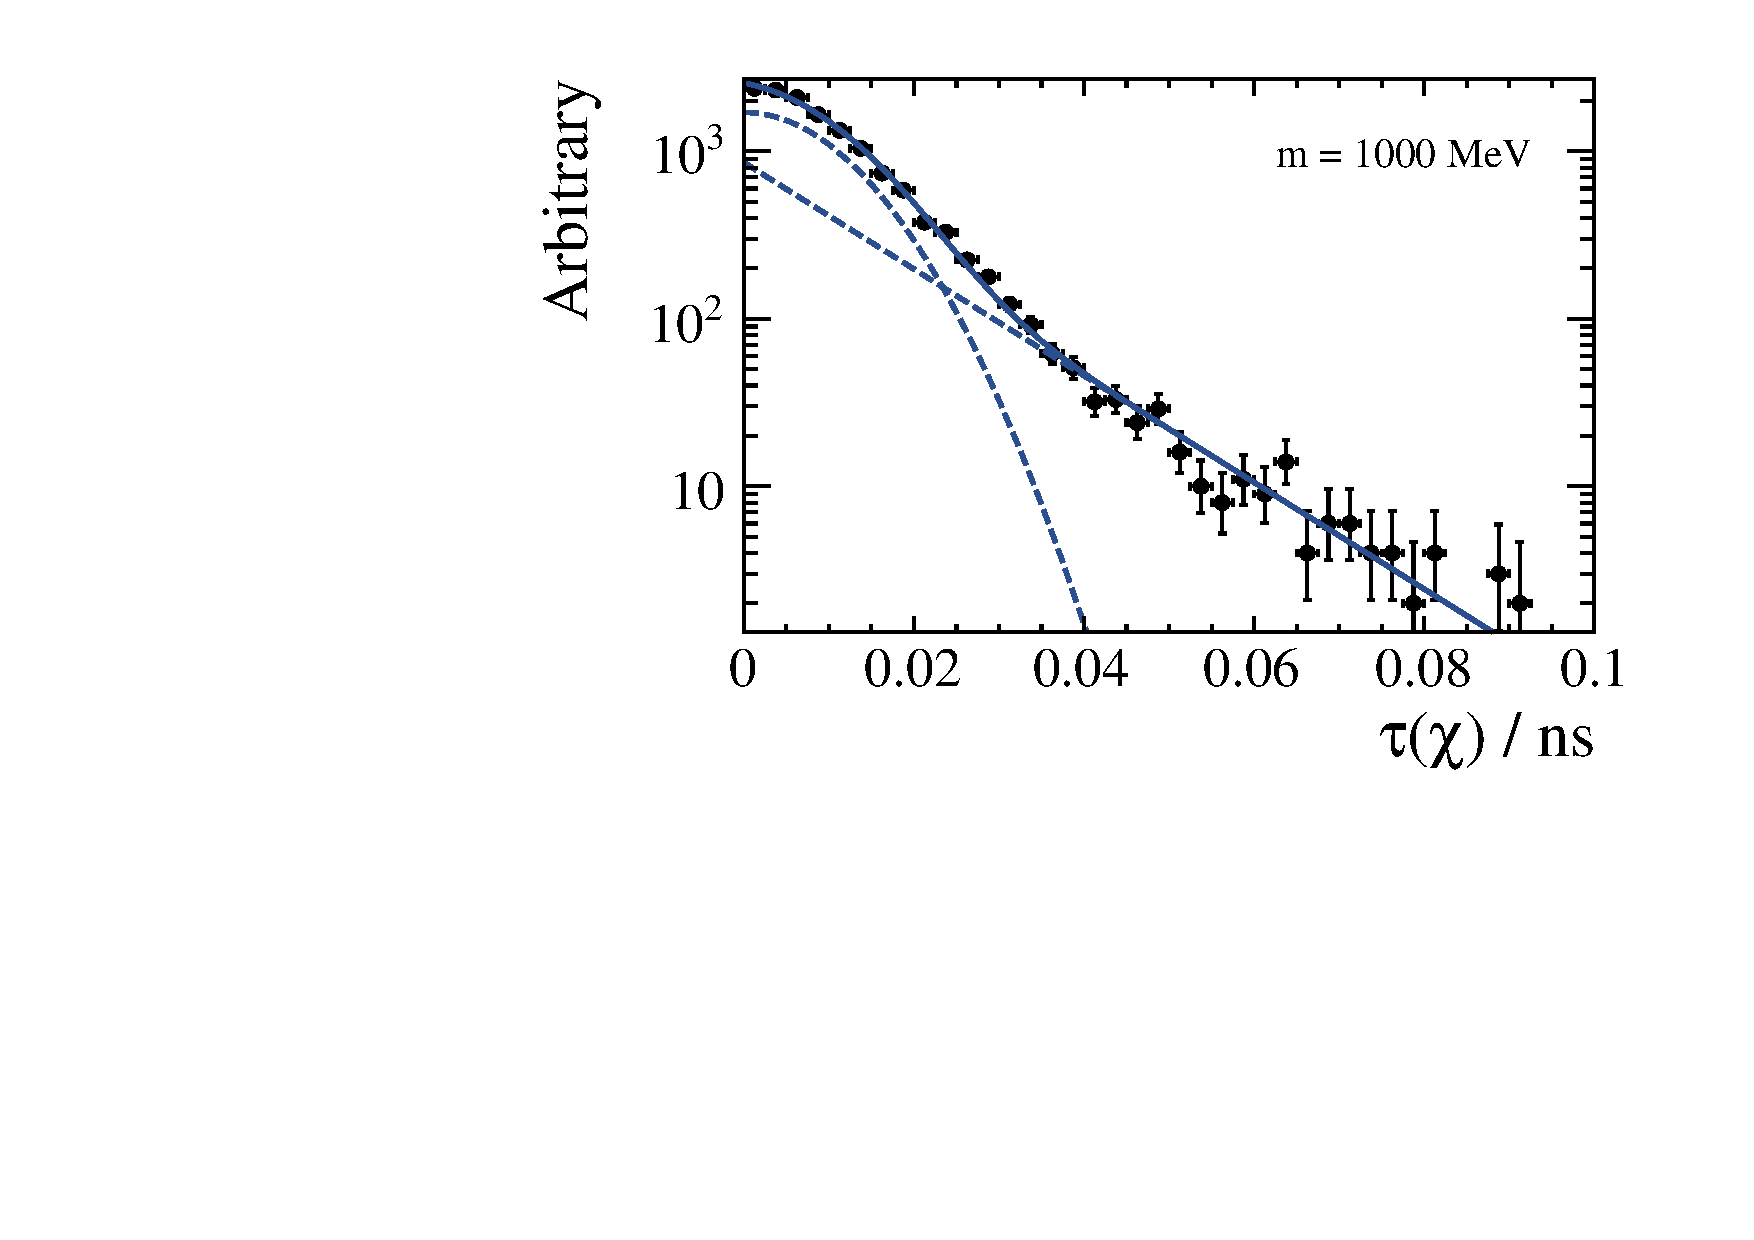
\includegraphics[width=0.48\textwidth]{anaTauEff_1000}
    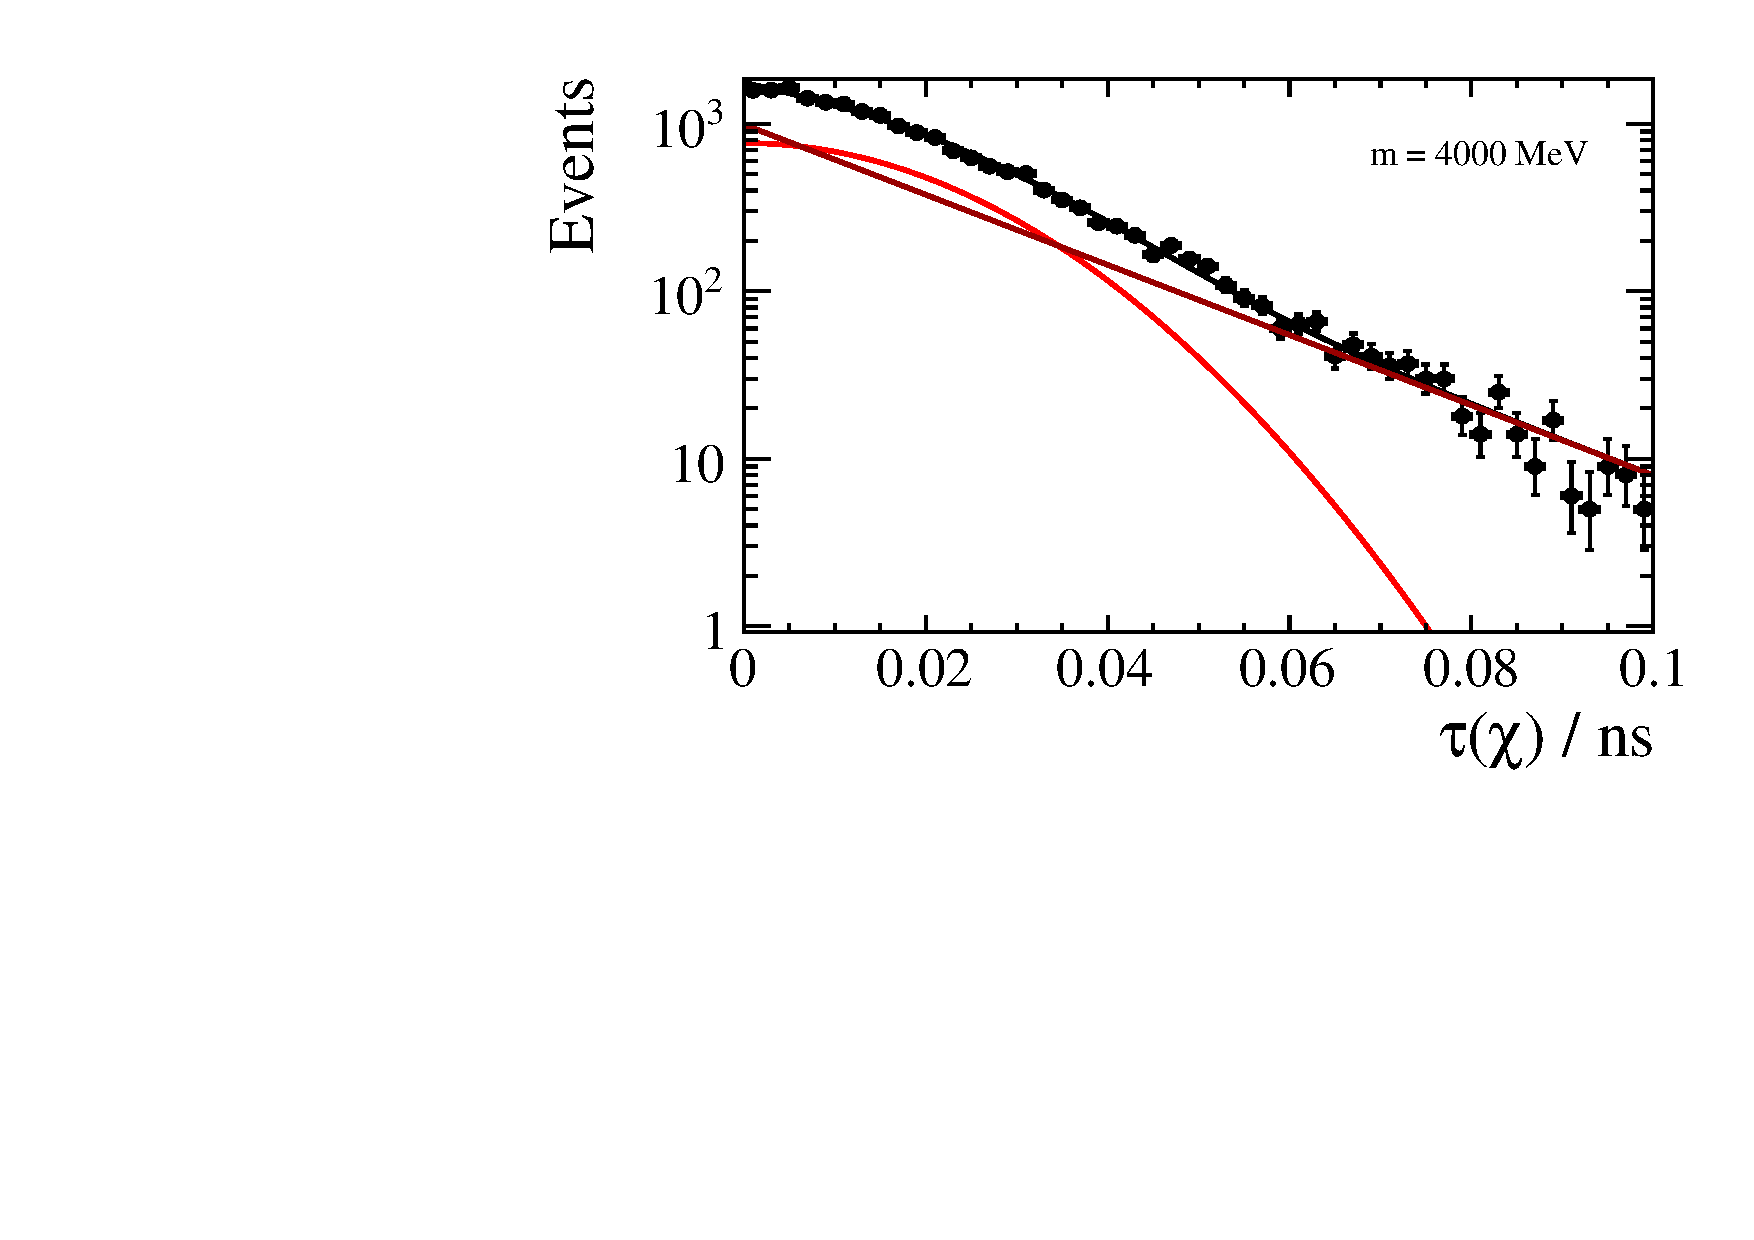
\includegraphics[width=0.48\textwidth]{anaTauEff_4000}
    \caption{\small
      Fits, using the function in Eq.~\protect\ref{eq:eff:parameters},
      to the lifetime distributions of simulated events produced with the masses:
      214, 250, 1000, and $4000\mev$ (as indicated)
      each with $\tau_\db=100\ps$.
      The black points are the simulated events, and the black line is the total fit, with light
      and dark red lines showing the Gaussian and exponential components, respectively.
    }
    \label{fig:eff:fits}
  \end{center}
\end{figure}

The parameters $\sigma$, and $\alpha$ are seen to evolve smoothly as a function of mass, and as
such spline interpolation is used to determine their values for arbitrary masses.
Linear regression is used to evolve $f$, because of the large errors on the values of $f$ yielded
by these fits.
Figure~\ref{fig:eff:spline} shows how the aforementioned parameters evolve as a function of mass.

\begin{figure}
  \begin{center}
    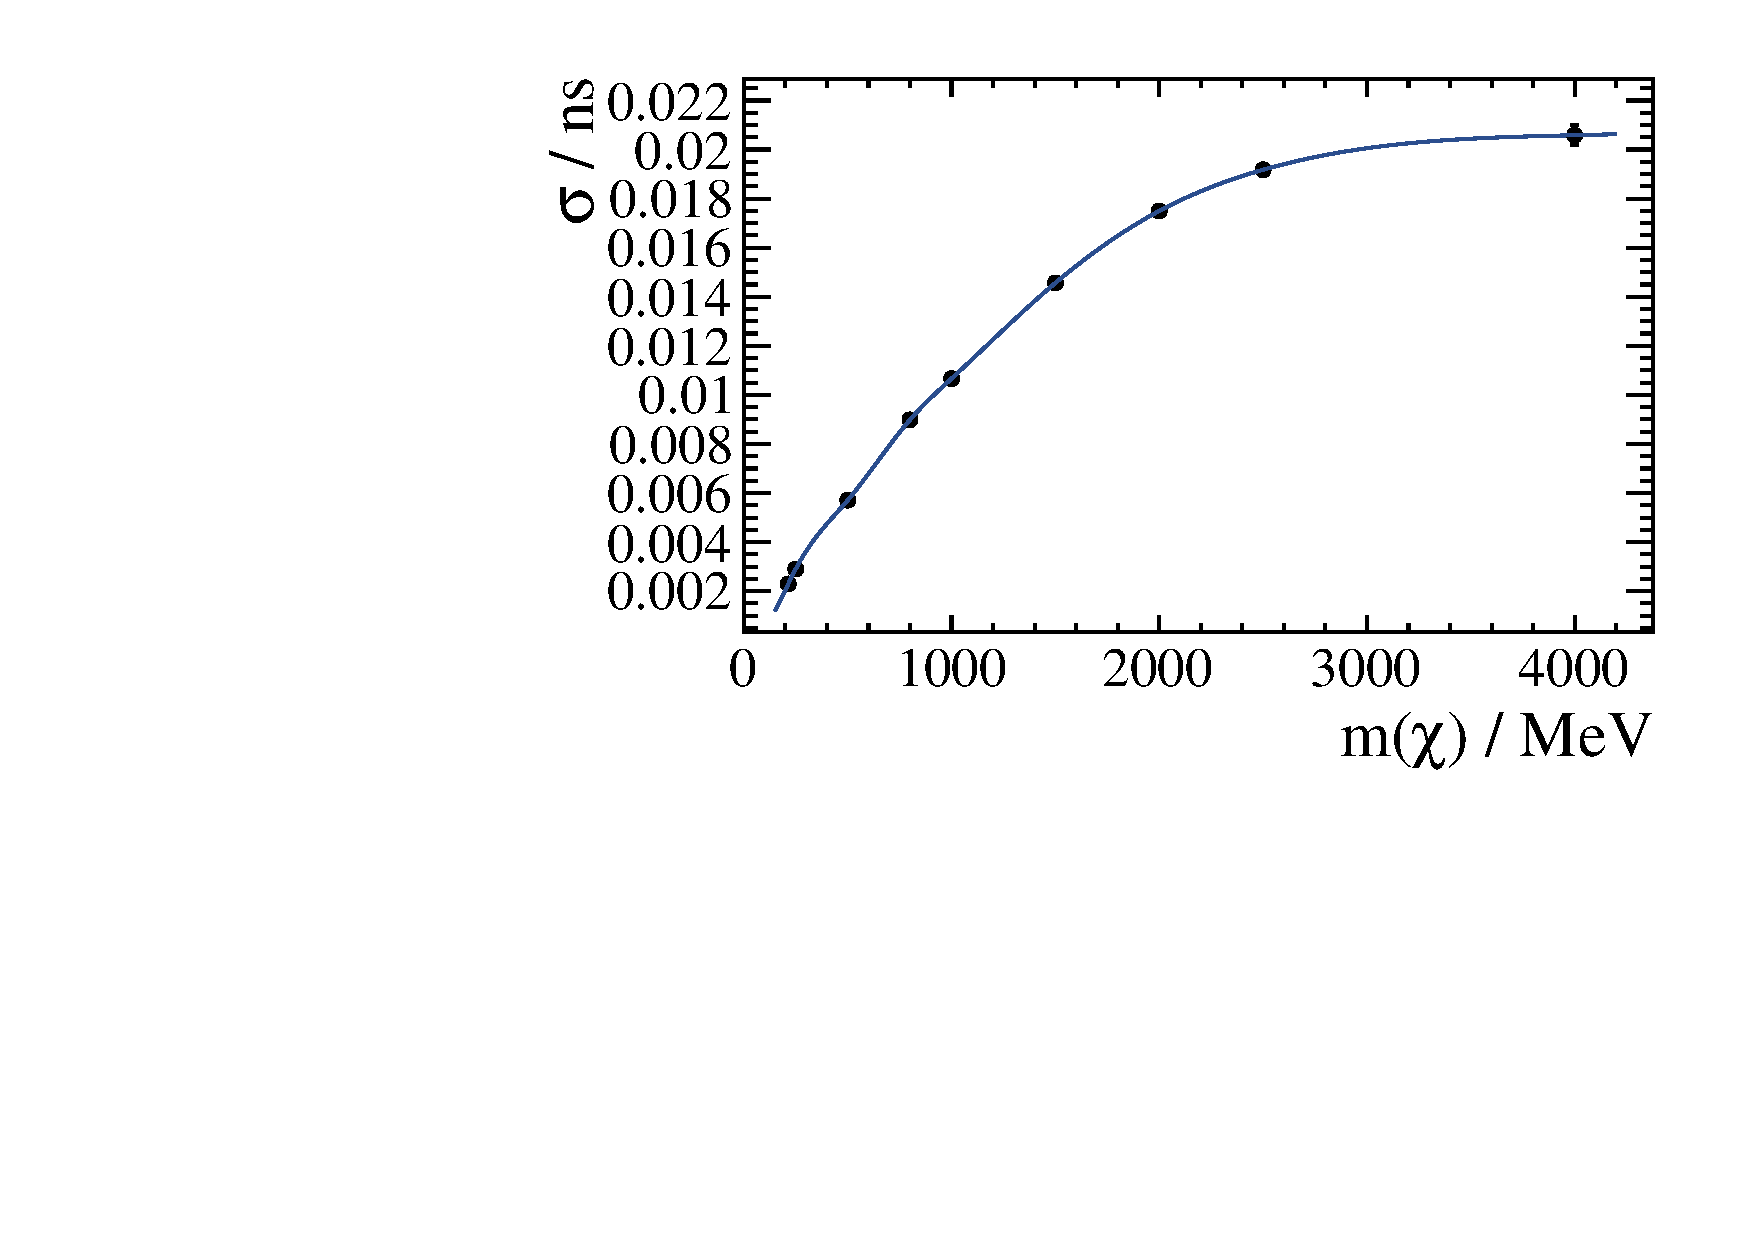
\includegraphics[width=0.48\textwidth]{spline_sigma}
    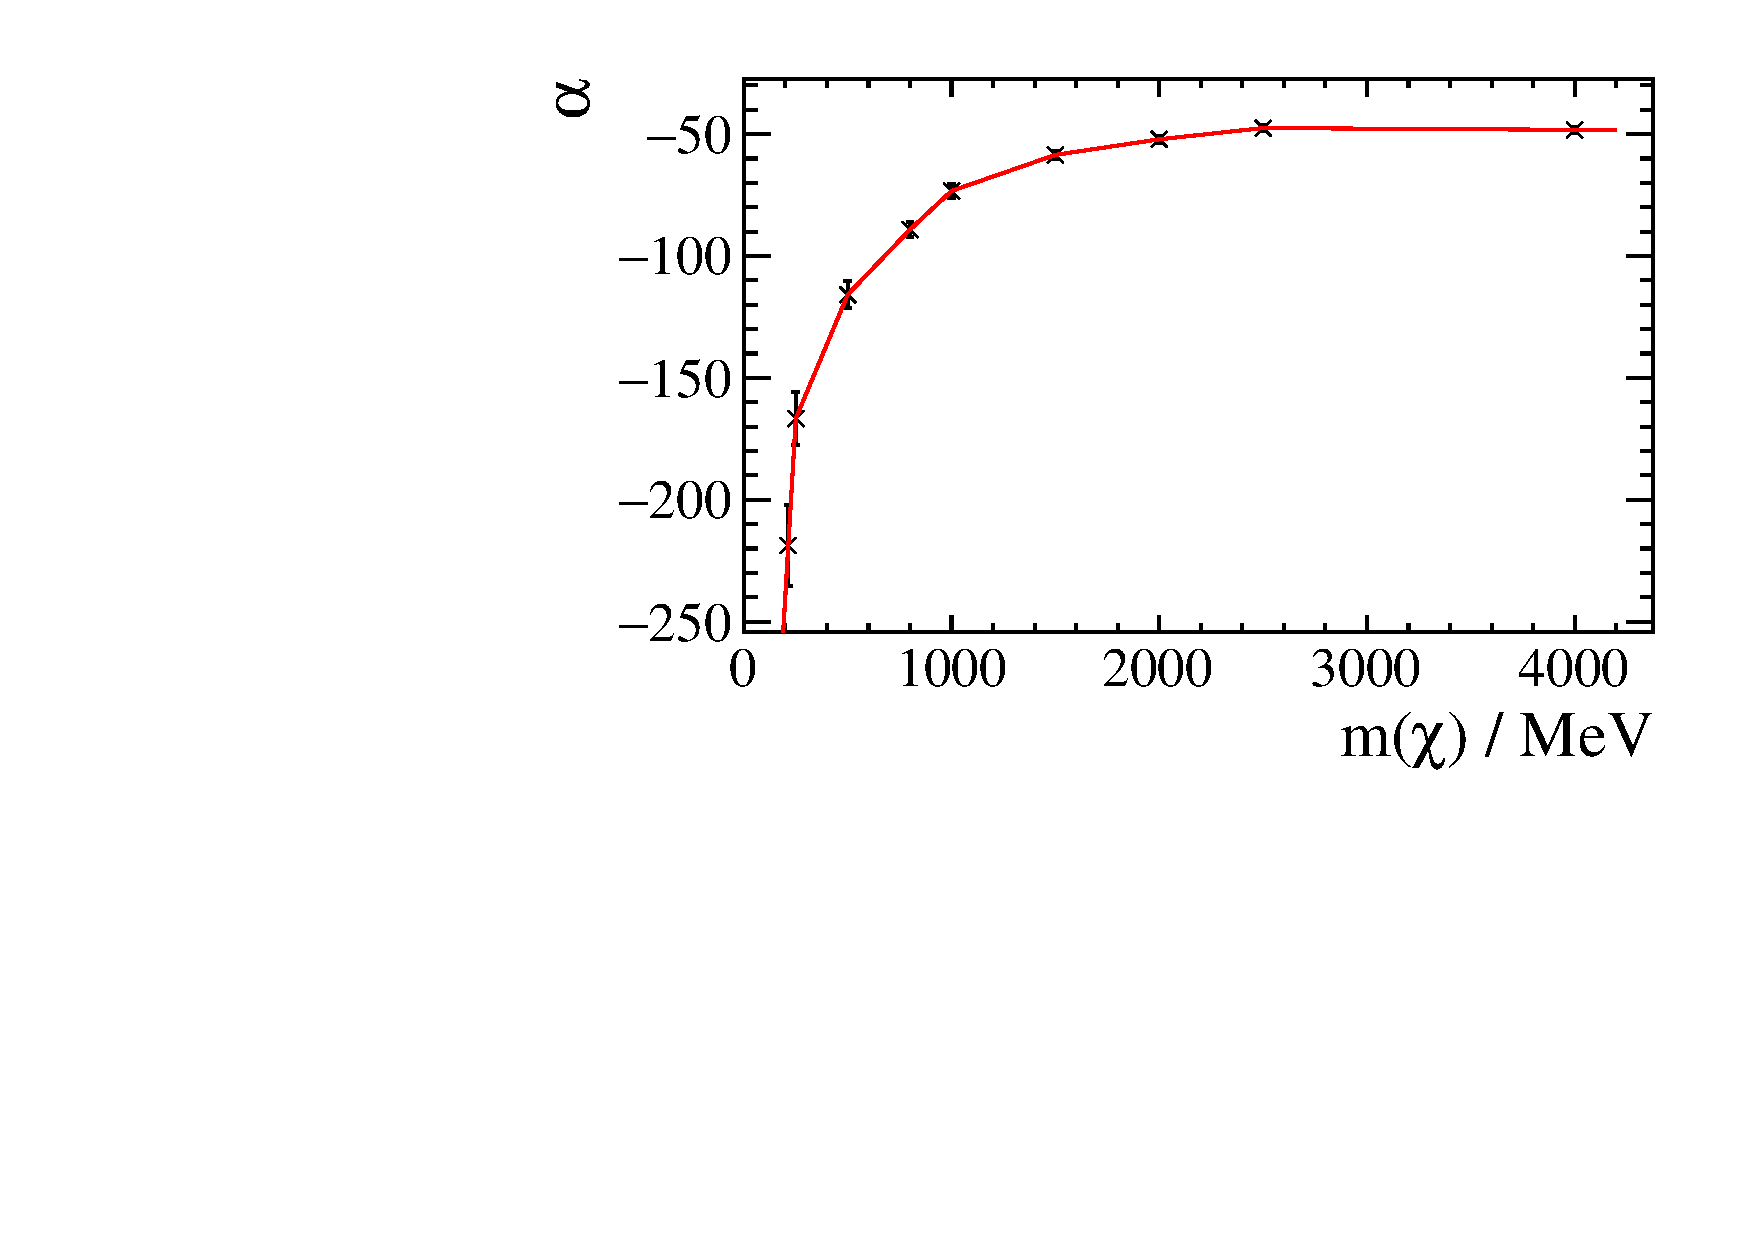
\includegraphics[width=0.48\textwidth]{spline_alpha}\\
    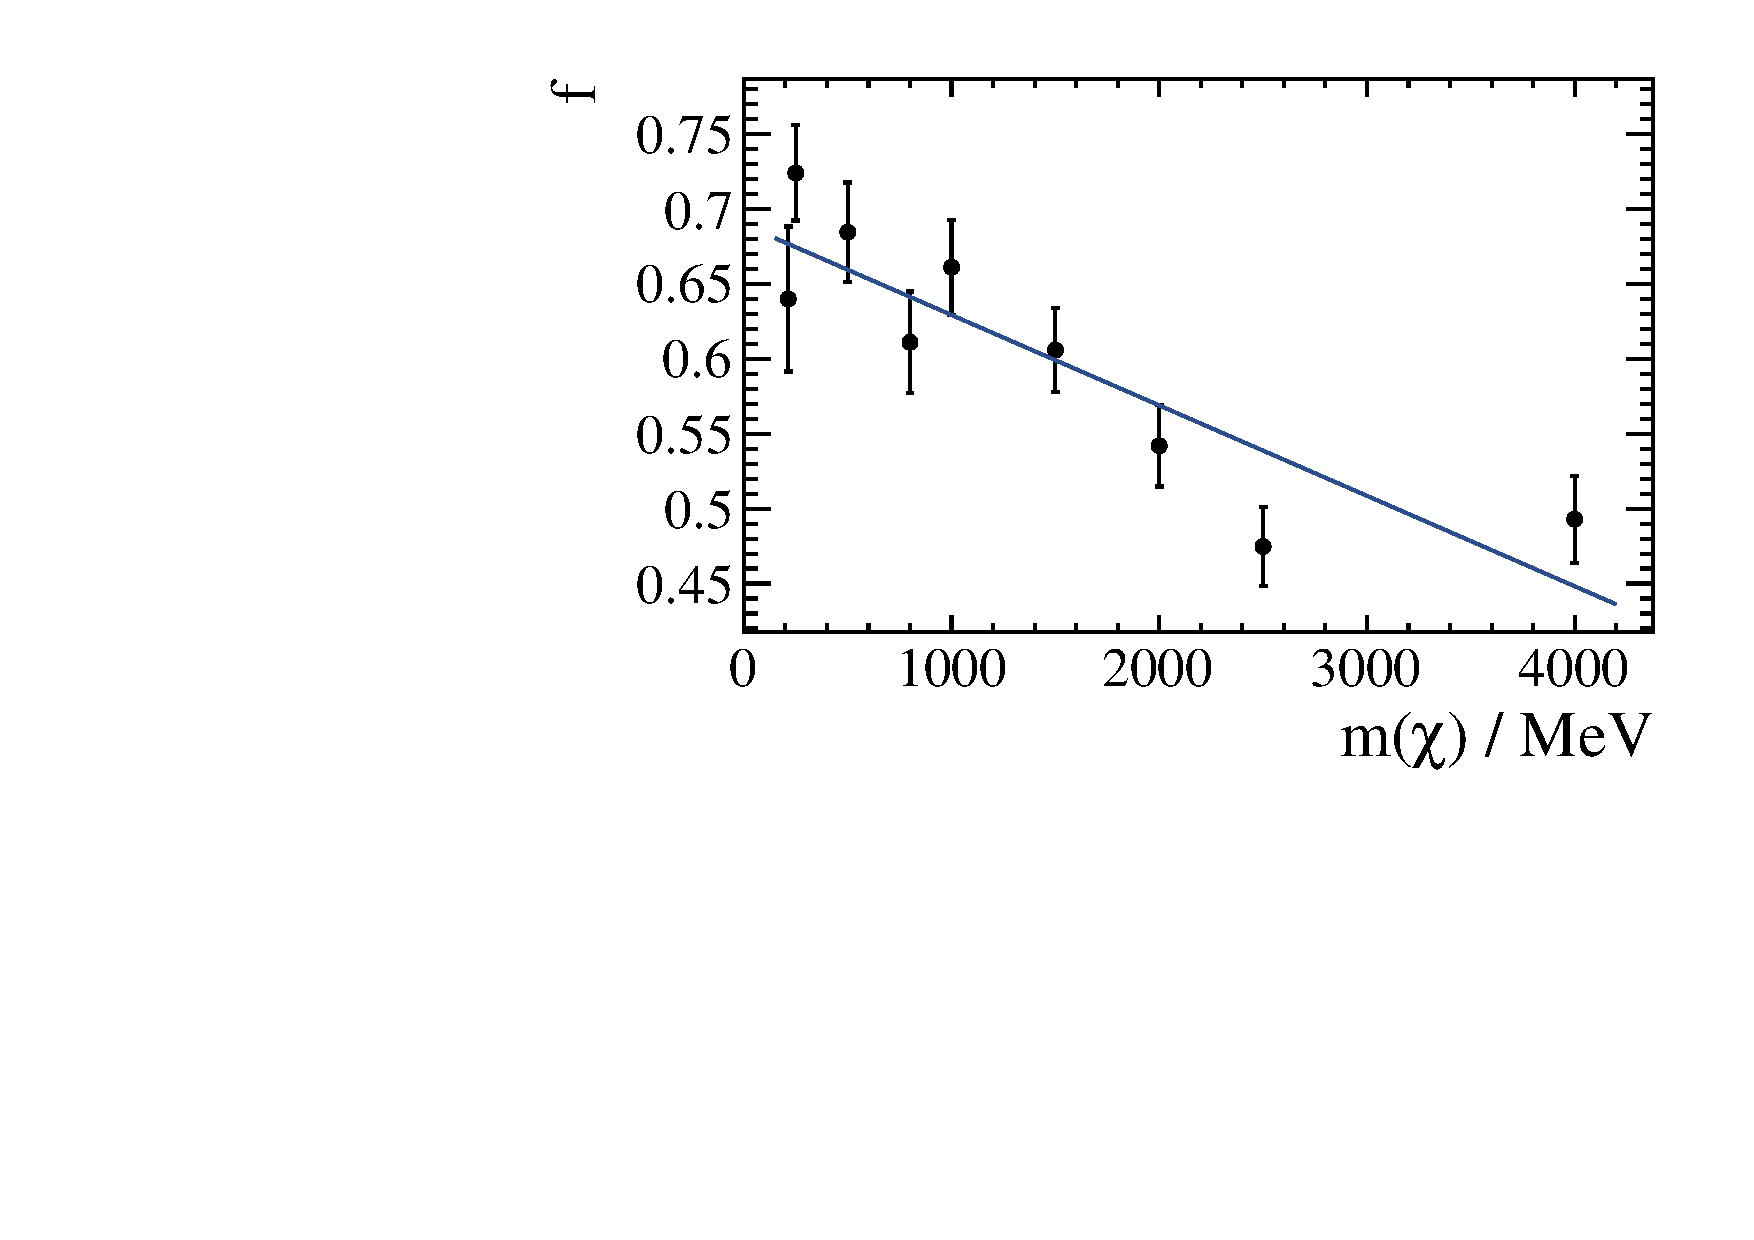
\includegraphics[width=0.48\textwidth]{spline_frac}
    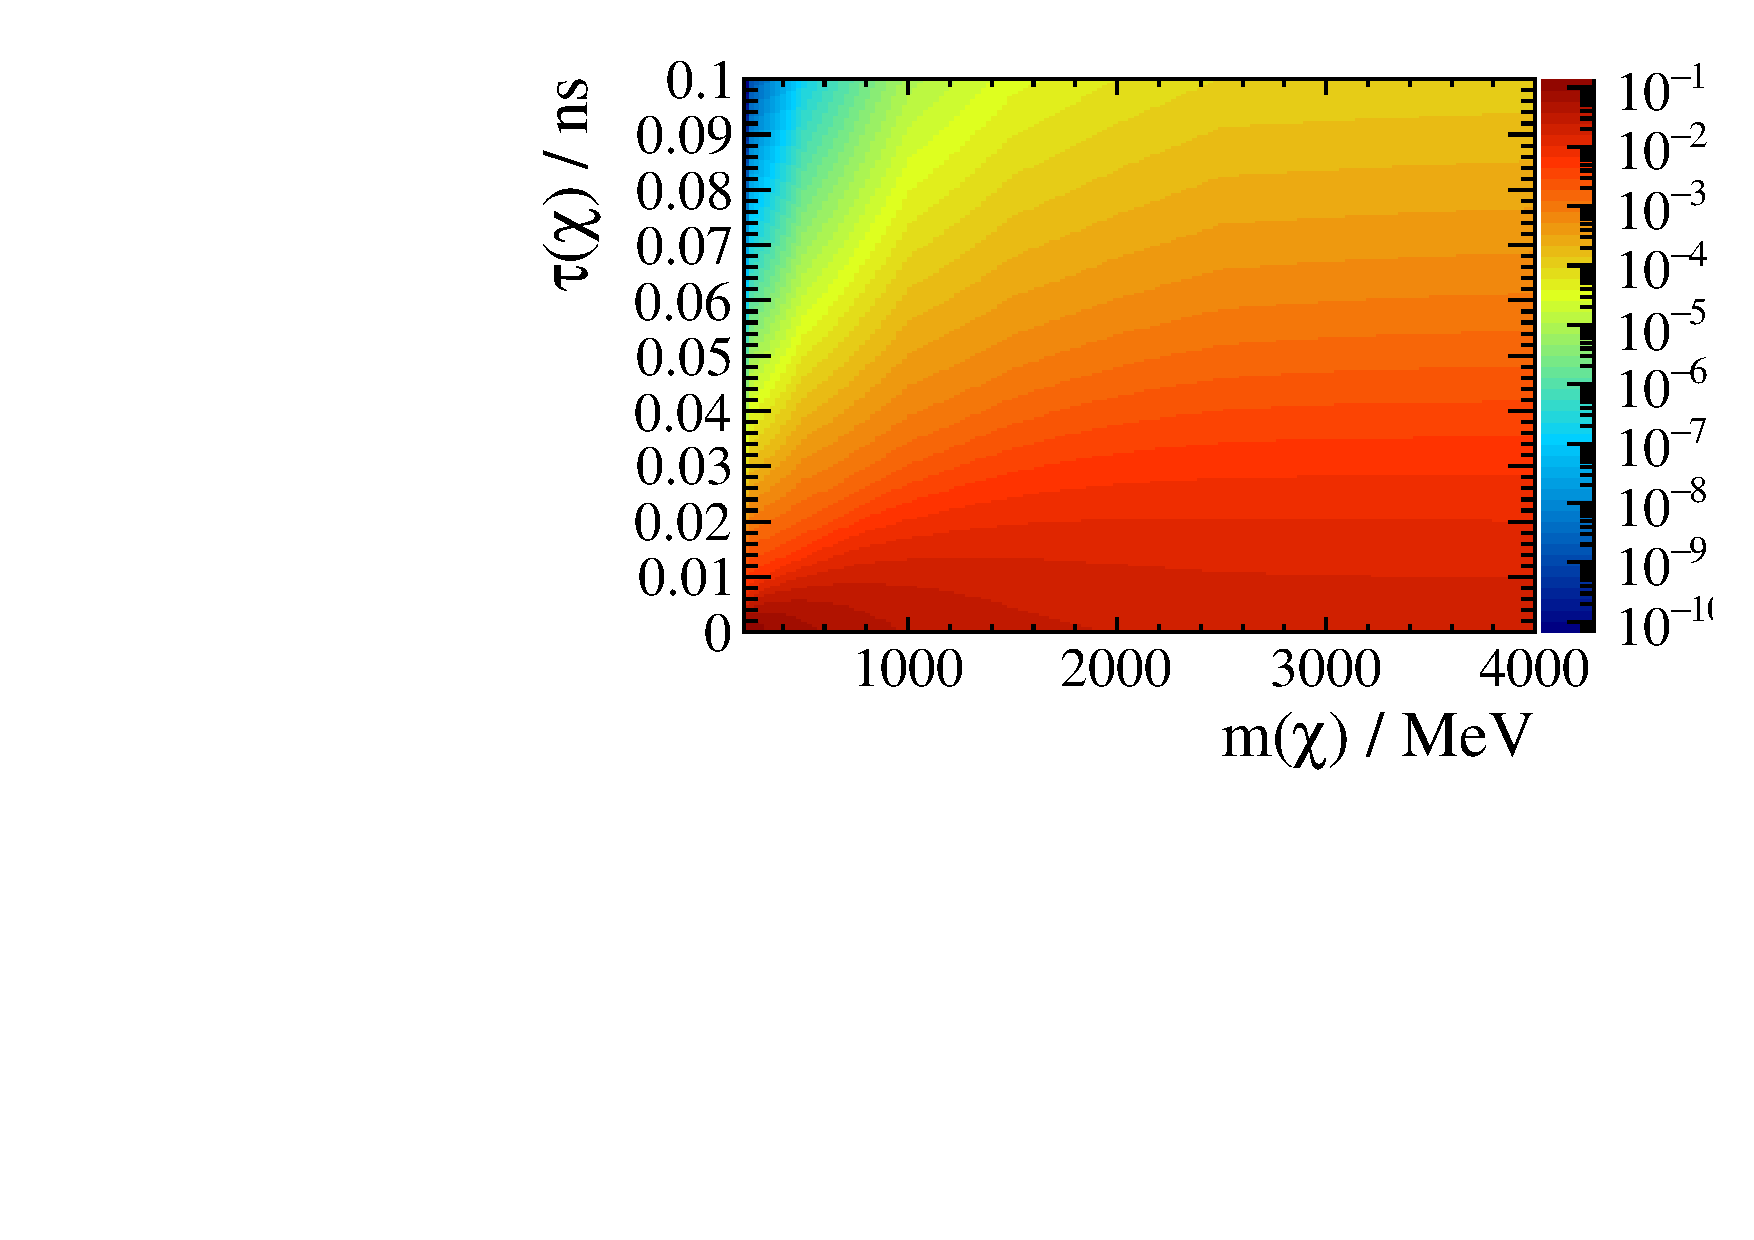
\includegraphics[width=0.48\textwidth]{spline_2d}
    \caption{
      Parameters from Eq.~\protect\ref{eq:eff:parameters} as a function of mass from
      simulated events.
      The parameters are
      (upper left) $\sigma$,
      (upper right) $\alpha$, and
      (lower) $f$.
      Splines are used to parameterize each shape, except for the parameter $f$, where a
      linear fit is used.
    }
    \label{fig:eff:spline}
  \end{center}
\end{figure}

%The two-dimensional map of parameterized lifetime distributions in \Fig{fig:eff:spline}
%Ratio of efficiency for a \db with $\lifetime{\db}=0\ps$

%\begin{figure}
  %\begin{center}
    %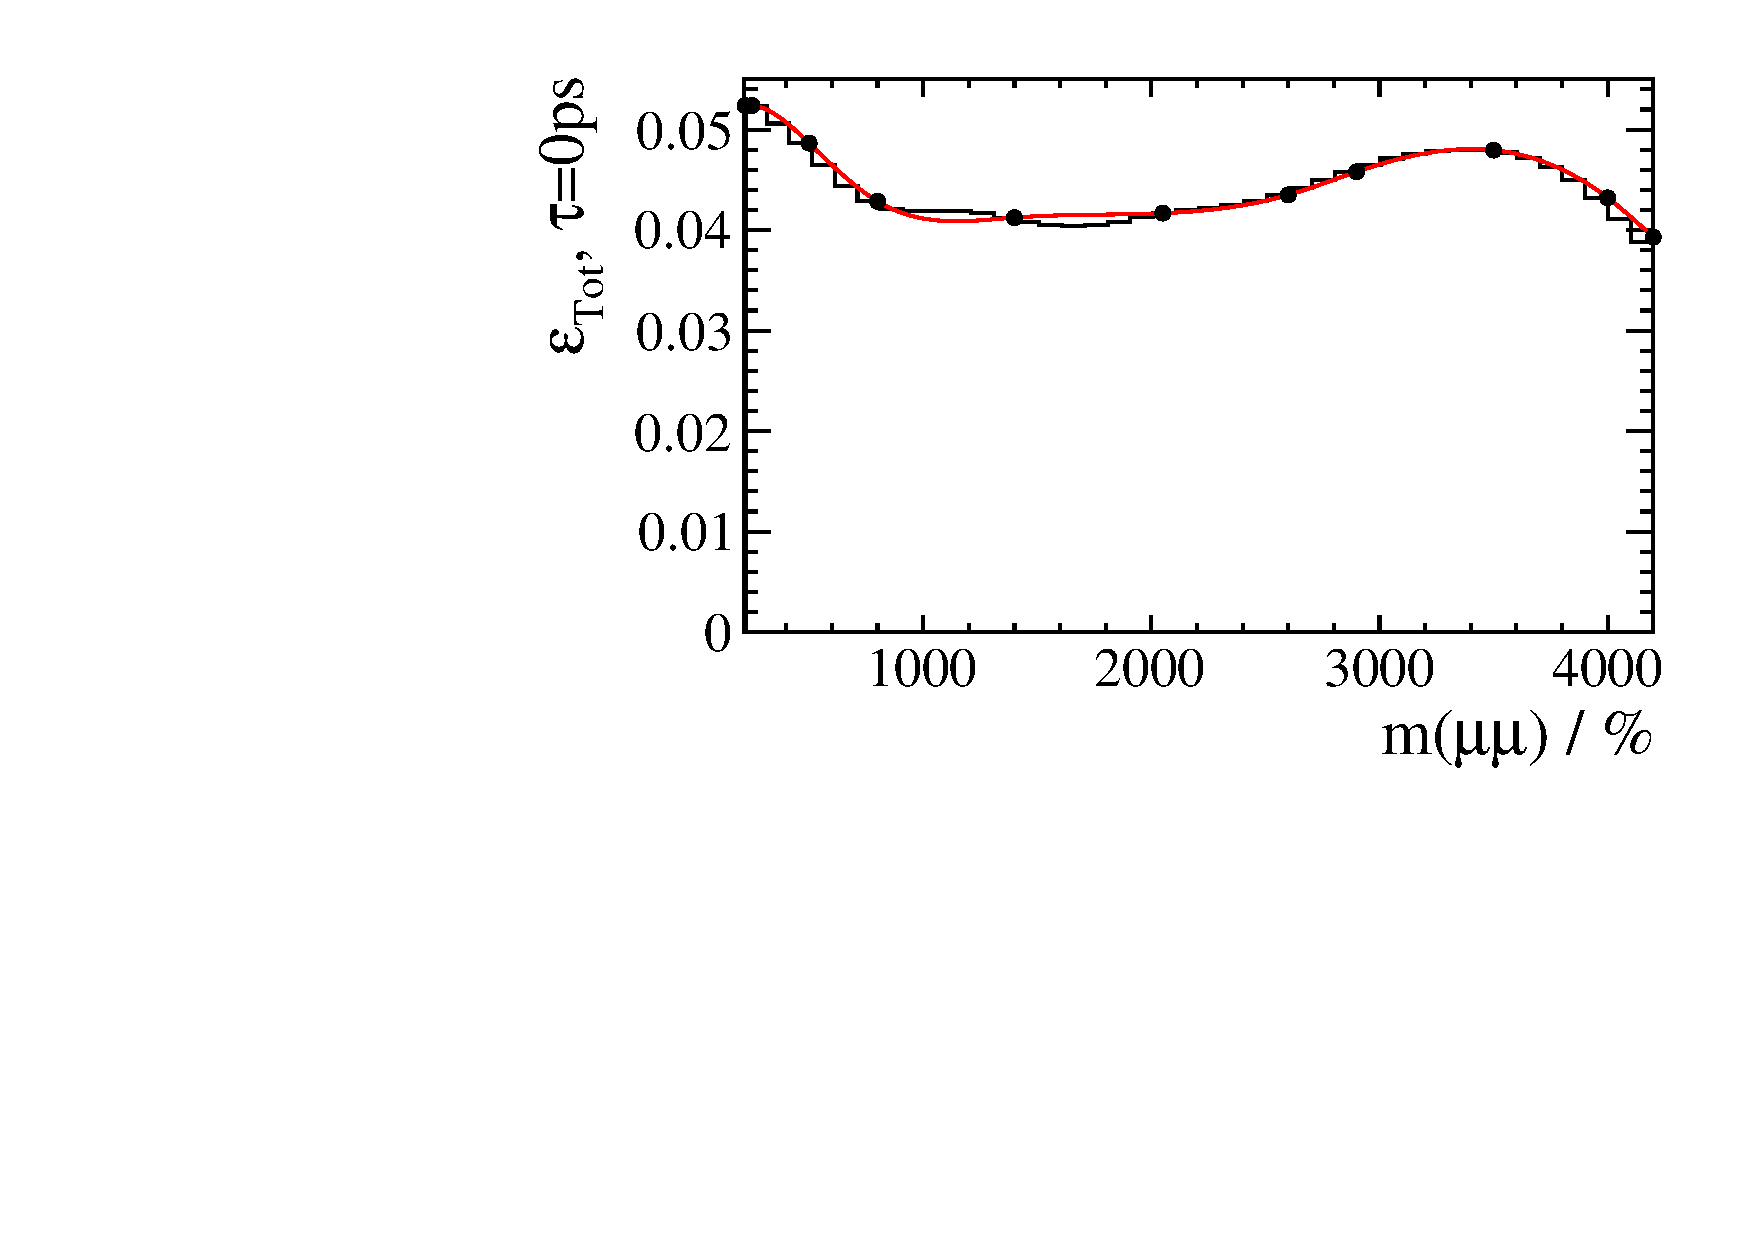
\includegraphics[width=0.48\textwidth]{kpieff.pdf}
    %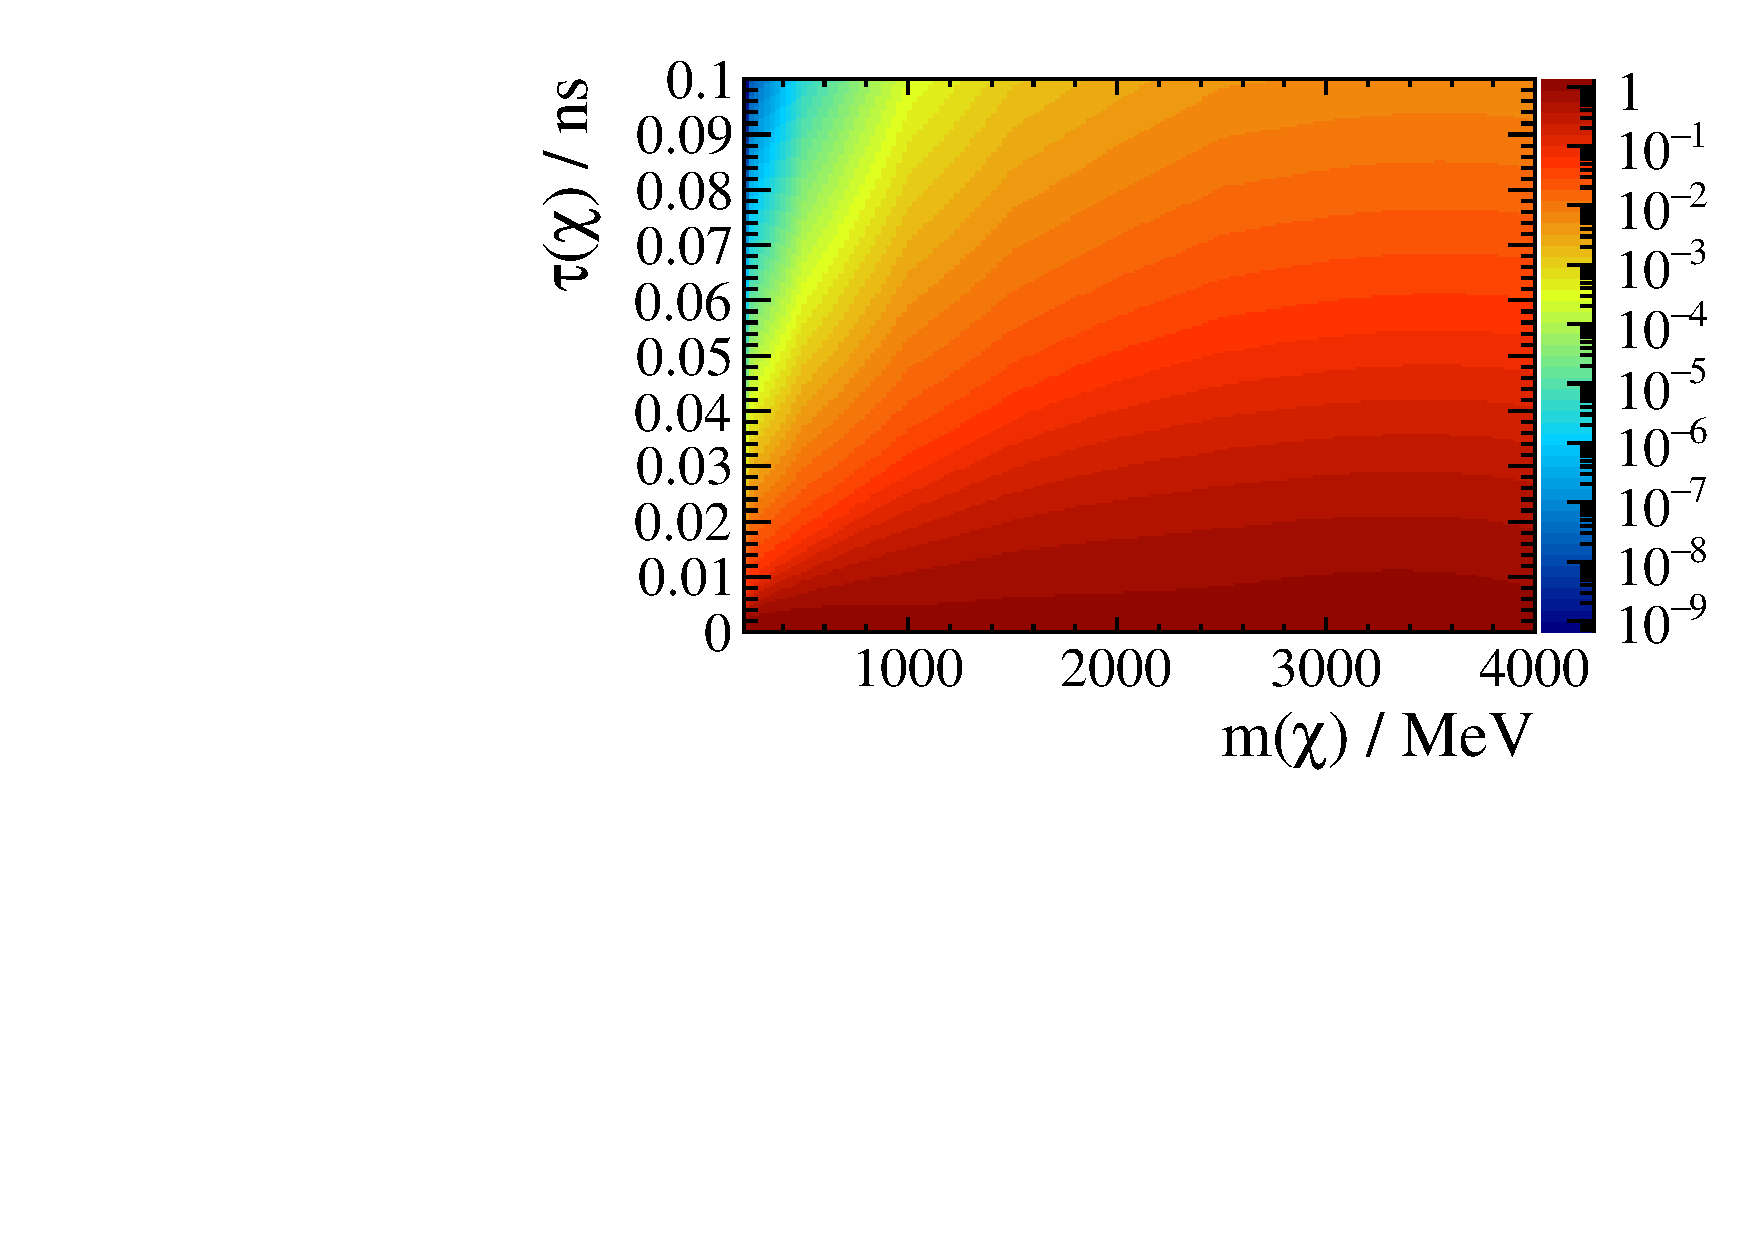
\includegraphics[width=0.48\textwidth]{spline_eff_2d}
    %\caption{
      %Using the parameters in Fig.~\ref{fig:eff:spline} and Eq.~\protect\ref{eq:eff:parameters} the
      %lifetime distributions are formed for the full two-dimensional projection.
      %Absolute efficiencies are not folded in here.
    %}
    %\label{fig:eff:effmap}
  %\end{center}
%\end{figure}



%Samples with different masses are fit with the results for each parameter plotted against dimuon
%mass in \Fig{fig:eff:spline}.
%Extrapolation to different masses is done using spline interpolation, as shown in
%\Fig{fig:eff:spline}.
%The value of $f$ has large errors, and has little effect on the total shape.
%A cubic spline models this very poorly because of the fluctuations at low mass, therefore linear
%regression is used instead.
%These splines account for all efficiencies except for the efficiency of the uBDT and the geometric
%acceptance of the \lhcb detector; the \uBDT and geometric acceptance are nearly the same for all
%samples and so nearly cancel in the limit setting.
%An example of a lifetime efficiency distribution for a given mass is shown in \Fig{fig:eff:effmap},
%as is the two-dimensional projection, absolute efficiencies have not been included in this.


By convolving the function $\mathcal{T}(\tau)$ with an exponential, the efficiency for any value of
lifetime can be derived:
\begin{equation}
  \varepsilon(\tau) =
  \frac{1}{\tau}\int\limits_0^{100\ps}
  \mathcal{T}(\tau^{\prime})
  \exp\left(-\frac{\tau^{\prime}}{\tau}\right)
  \,{\rm d}\tau^{\prime}.
\end{equation}
The upper lifetime acceptance is chosen to be $100\ps$, because the efficiency at longer lifetimes,
for all values of \mass{\db}, is very poor.




